%\documentclass[11pt,a4paper]{article}
\documentclass[11pt
  , a4paper
  , article
  , oneside
%  , twoside
%  , draft
]{memoir}

\usepackage{control}
\usepackage[numbers]{natbib}

\begin{document}

\newcommand{\technumber}{
  RAON Control-Document Series\\
  Revision : v1.0,   Release : a fixed date}
\title{\textbf{Raspberry Pi Technical Documentation}}

\author{scwook\thanks{@ibs.re.kr} \\

  Rare Isotope Science Project\\
  Institute for Basic Science, Daejeon, South Korea
}
\date{\today}

\renewcommand{\maketitlehooka}{\begin{flushright}\textsf{\technumber}\end{flushright}}
%\renewcommand{\maketitlehookb}{\centering\textsf{\subtitle}}
%\renewcommand{\maketitlehookc}{C}
%\renewcommand{\maketitlehookd}{D}

\maketitle

\begin{abstract}
본 메뉴얼에서는 Raspberry Pi에 대한 기본 설치 및 설정방법을 포함하여 다양한 센서들을 이용한 테스트 및 
EPICS Integration 방법에 대하여 설명하였다. 기본적으로 사용된 Model은 Raspberry Pi Model B+를 
이용하였다.\citep{FAI}
\end{abstract}

\chapter{Raspberry Pi}
Raspberry Pi(RPi)는 교육용 프로젝트의 일환으로 개발된 소형 컴퓨터로 가격이 아주 저렴하고 신용카드 정도의
크기를 가지고 있다.
\section{Hardware}
RPi는 5V의 Micro USB를 통해 전원을 공급받으며 USB, Ethernet Port, HDMI를 지원한다. 
특히 입출력 신호를 제어하기 위한 GPIO(General Purpose Inut Output)
포트를 지원하는데 SPI, I2C, UART통신이 가능하다.
\section{Software}
RPi에서 설치가능한 OS는 현제 
\section{Installation}
Raspbian을 설치하는 방법은 2가지가 있다.
\begin{itemize}
\item New Out Of the Box Software(NOOBS) 설치
\item Raspbian Image 설치
\end{itemize}
Raspberry Pi에 설치되는 OS는 Raspbian외에 몇가지가 더 있는데 NOOBS는 이러한 OS를 Package로 묶은 것으로 
하나 또는 그 이상의 OS를 한번에 설치할 수 있다. 만약 하나의 OS만 설치하고자 하는 경우에는 Image파일을 
이용하여 설치하면 된다. Raspberry 홈페이지에서는 NOOBS를 이용하는 것을 추천함으로 여기에서도 NOOBS를 
이용하여 설치를 진행하였다.
\subsection{Download}
Raspbian 설치를 위해 다음 홈페이지에서 NOOBS 파일을 다운 받는다\\
http://www.raspberrypi.org/downloads/\\
다운로드한 파일의 압축을 해제한다. Micro SD Card를 PC에 연결한 후 압축해제한\\ 
NOOBS 파일을 전부 복사한다.
PC에서 Micro SD Card를 제거한 후 Raspberry Pi에 연결한다.
\subsection{First Boot}
Raspberry Pi전원을 연결 하면 NOOBS Install Manager가 나온다.
Raspbian을 선택한 후(2번 째 있는걸 선택) Install 버튼을 눌러 설치를 진행한다.
설치 완료 버튼을 누르면 자동으로 재부팅 된다.
부팅이 완료되면 Raspberry Pi Software Configuration Tool이 나타나는데 Finish를 눌러 설치를 완료한다.
\section{Configuration}
\subsection{Host Name 및 Password 변경}

\subsection{Networking}

\section{Library}
\subsection{wiringPi}
Raspberry Pi는 입출력 신호 제어를 위해 다음과 같은 40pin(Model B의 경우 26pin) 포트를 제공하고 있다.
Wiring Pi 설치는 git 서버로 부터 파일을 복사한 후 빌드하면 된다.
\begin{lstlisting}[style=termstyle]
pi@raspberry# git clone git://git.drogon.net/wiringPi
Cloning into 'wiringPi'...
remote: Counting objects: 657, done.
remote: Compressing objects: 100% (599/599), done.
remote: Total 657 (delta 476), reused 95 (delta 58)
Receiving objects: 100% (657/657), 247.61 KiB | 94 KiB/s, done.
Resolving deltas: 100% (476/476), done.
pi@raspberrypi# cd wiringPi
pi@raspberrypi:/wiringPi# ./build
\end{lstlisting}
Pin Layout은 'readall' 명령으로 확인 가능하다. Wiring Pi는 자체적인 Pin Map을 사용하는데 wPi로 표시된 부분은 Wiring Pi에서 사용하는 GPIO 핀 번호이다.
\begin{lstlisting}[style=termstyle]
pi@raspberrypi# gpio readall
+-----+-----+---------+------+---+--B Plus--+---+------+---------+-----+-----+
 | BCM | wPi |   Name  | Mode | V | Physical | V | Mode | Name    | wPi | BCM |
 +-----+-----+---------+------+---+----++----+---+------+---------+-----+-----+
 |     |     |    3.3v |      |   |  1 || 2  |   |      | 5v      |     |     |
 |   2 |   8 |   SDA.1 |   IN | 1 |  3 || 4  |   |      | 5V      |     |     |
 |   3 |   9 |   SCL.1 |   IN | 1 |  5 || 6  |   |      | 0v      |     |     |
 |   4 |   7 | GPIO. 7 |   IN | 0 |  7 || 8  | 1 | ALT0 | TxD     | 15  | 14  |
 |     |     |      0v |      |   |  9 || 10 | 1 | ALT0 | RxD     | 16  | 15  |
 |  17 |   0 | GPIO. 0 |   IN | 0 | 11 || 12 | 0 | IN   | GPIO. 1 | 1   | 18  |
 |  27 |   2 | GPIO. 2 |   IN | 0 | 13 || 14 |   |      | 0v      |     |     |
 |  22 |   3 | GPIO. 3 |   IN | 0 | 15 || 16 | 0 | IN   | GPIO. 4 | 4   | 23  |
 |     |     |    3.3v |      |   | 17 || 18 | 0 | IN   | GPIO. 5 | 5   | 24  |
 |  10 |  12 |    MOSI |   IN | 0 | 19 || 20 |   |      | 0v      |     |     |
 |   9 |  13 |    MISO |   IN | 0 | 21 || 22 | 0 | IN   | GPIO. 6 | 6   | 25  |
 |  11 |  14 |    SCLK |   IN | 0 | 23 || 24 | 0 | IN   | CE0     | 10  | 8   |
 |     |     |      0v |      |   | 25 || 26 | 0 | IN   | CE1     | 11  | 7   |
 |   0 |  30 |   SDA.0 |   IN | 0 | 27 || 28 | 0 | IN   | SCL.0   | 31  | 1   |
 |   5 |  21 | GPIO.21 |   IN | 0 | 29 || 30 |   |      | 0v      |     |     |
 |   6 |  22 | GPIO.22 |   IN | 0 | 31 || 32 | 0 | IN   | GPIO.26 | 26  | 12  |
 |  13 |  23 | GPIO.23 |   IN | 0 | 33 || 34 |   |      | 0v      |     |     |
 |  19 |  24 | GPIO.24 |   IN | 0 | 35 || 36 | 0 | IN   | GPIO.27 | 27  | 16  |
 |  26 |  25 | GPIO.25 |   IN | 0 | 37 || 38 | 0 | IN   | GPIO.28 | 28  | 20  |
 |     |     |      0v |      |   | 39 || 40 | 0 | IN   | GPIO.29 | 29  | 21  |
 +-----+-----+---------+------+---+----++----+---+------+---------+-----+-----+
 | BCM | wPi |   Name  | Mode | V | Physical | V | Mode | Name    | wPi | BCM |
 +-----+-----+---------+------+---+--B Plus--+---+------+---------+-----+-----+
\end{lstlisting}

\begin{figure}
  \centering
  \subbottom[Model B]
  {
    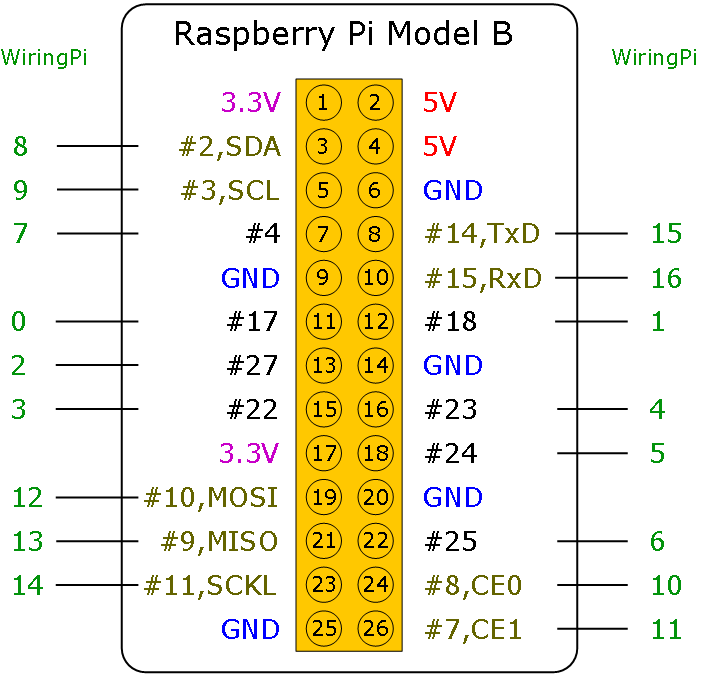
\includegraphics[width=175px]{./images/raspberry/pinmapb.png}
    \label{fig:pin_b}
  }
  \hfill
  \subbottom[Model B+]
  {
    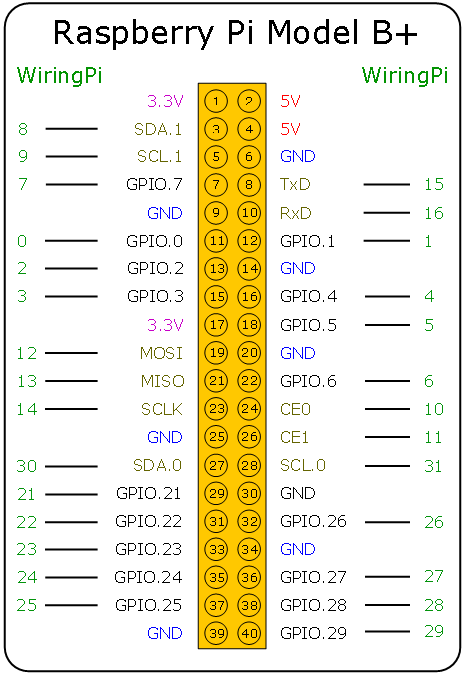
\includegraphics[width=116px]{./images/raspberry/pinmapbp.png}
    \label{fig:pin_bp}
  }
  \caption{Raspberry Pi Pin Map}
  \label{fig:rpi_pin_map}
\end{figure}

\chapter{Application}
본 Chapter에서는 RPi에 연결 가능한 Device 및 Sensor를 이용한 테스트 설명한다. 테스트는 Model B+에서
진행되었으며 기본적으로 Rasbian 과 wiringPi가 설치되어 있어야한다.
\section{Pi Camera}
Raspberry Pi에서 제공하고 있는 카메라는 2종류가 있다. 하나는 일반적으로 사용하는 카메라로 기판 색이 
초록색으로 되어 있다. 다른 하나는 NoIR(No Infrared) 카메라로 기판색이 검은색으로 되어 있다. 두 카메라는 
기능적으로 완전 동일하나 NoIR 카메라는 적외선 필터가 없으므로 적외선 영역까지도 볼 수있다. 
즉 적외선 LED와 함께 사용하면 어두운 장소에서도 촬영이 가능하다. 반면 낮에는 실제 색감 및 밝기가 일반
카메라와 다르게 보이는 단점이 있다.
\begin{figure}
  \centering
  \subbottom[Normal Camera] 
  {
    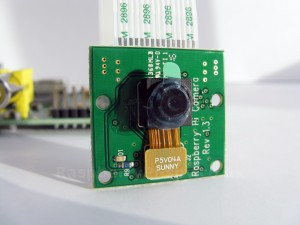
\includegraphics[width=0.47\textwidth]{./images/raspberry/camera.jpg}
    \label{fig:nor_cam}
  }
  \hfill
  \subbottom[NoIR Camera]
  {
    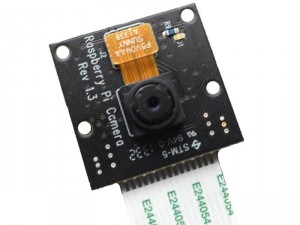
\includegraphics[width=0.47 \textwidth]{./images/raspberry/noircamera.jpg}
    \label{fig:noir_cam}
  }
  \caption{Raspberry Pi Camera Module}
  \label{fig:rpi_cam}
\end{figure}

\subsection{Installation}
RPi 카메라 모듈은 Figure \ref{fig:ist_cam}과 같이 Camera 전용 Port를 사용하며 RPi Configuration
을 통해 Port를 활성화 시켜 준다.
\begin{figure}[!htb]
\centering
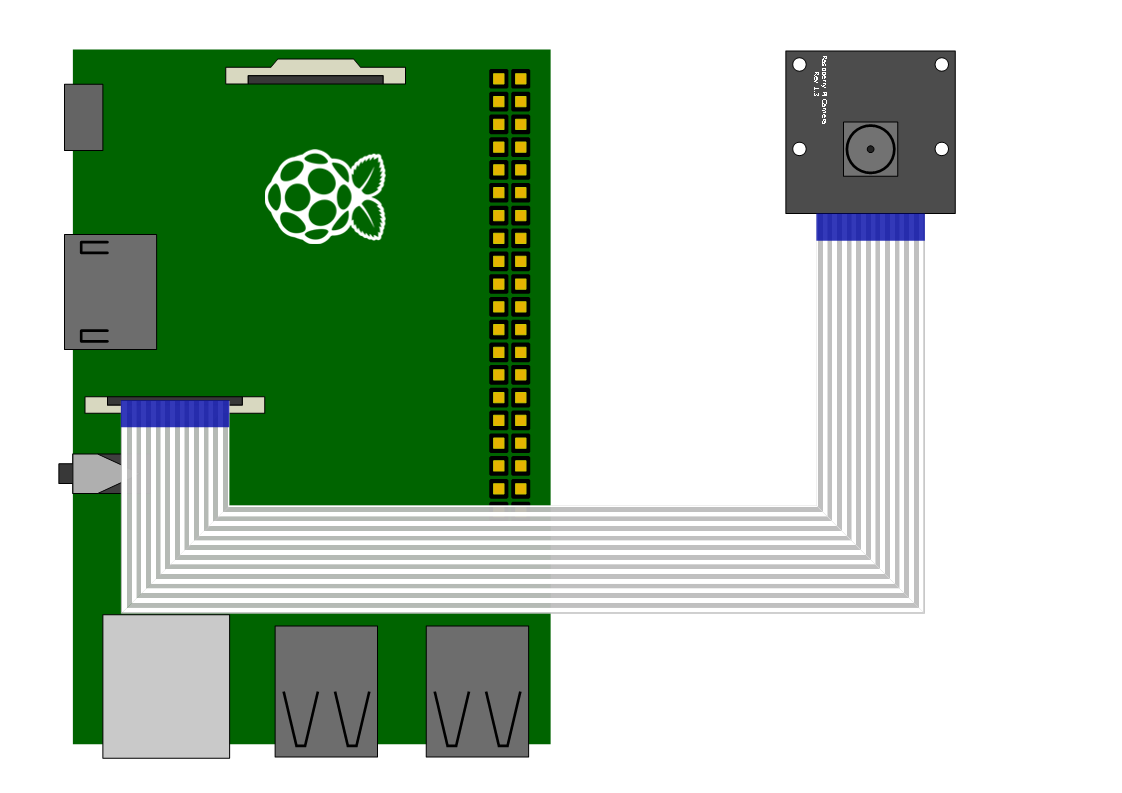
\includegraphics[width=1\textwidth]{./images/raspberry/pi_camera_setting.png}
\caption{Camera Installation}
\label{fig:ist_cam}
\end{figure}
\begin{lstlisting}[style=termstyle]
pi@raspberry# sudo raspi-config
\end{lstlisting}
\begin{figure}[!htb]
\centering
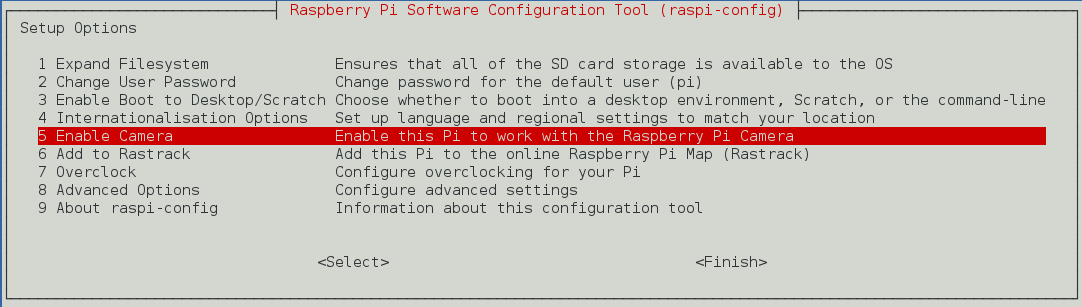
\includegraphics[width=1\textwidth]{./images/raspberry/enable_camera.png}
\caption{Camera Installation}
\label{fig:en_cam}
\end{figure}
\begin{figure}[!htb]
\centering
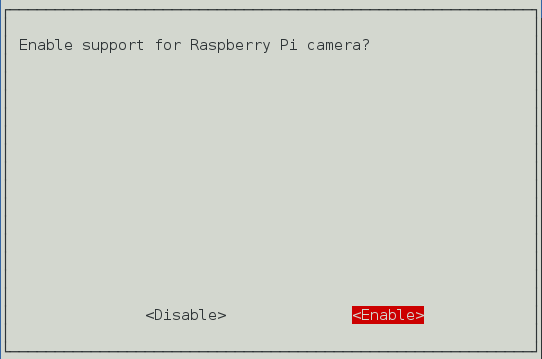
\includegraphics[width=1\textwidth]{./images/raspberry/enable_camera_sel.png}
\caption{Camera Installation}
\label{fig:sel_en_cam}
\end{figure}
설정을 마쳤으면 재부팅 한다.
\begin{lstlisting}[style=termstyle]
pi@raspberry# sudo reboot
\end{lstlisting}
\subsection{Test}
기본적인 카메라 사용방법은 다음과 같다.\\
사진 캡쳐는 raspitill을 사용한다.
\begin{lstlisting}[style=termstyle]
pi@raspberry# raspistill -o cam.jpg
\end{lstlisting}
상하 좌우 반전을 하고 싶으면 vf, hf 옵션을 설정한다.
\begin{lstlisting}[style=termstyle]
pi@raspberry# raspivid -o vid.h264
\end{lstlisting}
t옵션을 사용하면 시간 설정이 가능하다.(기본은 5초) 다음은 10초동안 촬영한다.
\begin{lstlisting}[style=termstyle]
pi@raspberry# sudo raspi-config
\end{lstlisting}
카메라가 작동할 때 LED가 켜지지 않게 하려면 /boot/config.txt 파일에 disable\_camera\_led=1을 
추가한 후 재부팅 한다.
\begin{lstlisting}[style=termstyle]
...
...
...

# NOOBS Auto-generated Settings:
hdmi_force_hotplug=1
config_hdmi_boost=4
overscan_left=24
overscan_right=24
overscan_top=16
overscan_bottom=16
disable_overscan=0
start_x=1
gpu_mem=128
disable_camera_led=1
\end{lstlisting}
\subsection{Web Streaming}
Raspberry Pi Camera를 Web에서 볼 수 있도록 설정해 본다.
기본적인 설정은 다음 홈페이지를 따랐다.
http://www.rasplay.org/?p=7174
우선 필요한 Library를 설치한다.
\begin{lstlisting}[style=termstyle]
pi@raspberry# sudo apt-get install git cmake libjpeg8-dev imagemagick -y
\end{lstlisting}
다음 videodev.h 헤더파일을 videodev2.h파일로 링크한다.
\begin{lstlisting}[style=termstyle]
pi@raspberry# sudo ln -s /usr/include/linux/videodev2.h /usr/include/linux/videodev.h
\end{lstlisting}
\begin{lstlisting}[style=termstyle]
pi@raspberry# git clone https://github.com/jacksonliam/mjpg-streamer
\end{lstlisting}
다운 받은 코드를 make 한다.
\begin{lstlisting}[style=termstyle]
pi@raspberrypi# cd mjpg-streamer/mjpg-streamer-experimental
pi@raspberrypi:/mjpg-streamer/mjpg-streamer-experimental# make
\end{lstlisting}
make가 완료되면 다음과 같은 실행 스크립트를 만든다.
\begin{lstlisting}[style=termstylenumber, caption={Editing \texttt{/etc/fai/NFSROOT}}, label={list:nfsroot-file}]
export STREAMER_PATH=$HOME/mjpg-streamer/mjpg-streamer-experimental
export LD_LIBRARY_PATH=$STREAMER_PATH
$STREAMER_PATH/mjpg_streamer -i "input_raspicam.so -x 640 -y 480 -fps 30" -o "output_http.so -w $STREAMER_PATH/www"
\end{lstlisting}
스크립트를 실행 한다.
\begin{lstlisting}[style=termstyle]
pi@raspberrypi# sh mjpg.sh
MJPG Streamer Version: svn rev:
 DBG(/home/pi/mjpg-streamer/mjpg-streamer-experimental/plugins/input_raspicam/input_raspicam.c, input_init(), 118): argv[0]=raspicam 
input plugin
 DBG(/home/pi/mjpg-streamer/mjpg-streamer-experimental/plugins/input_raspicam/input_raspicam.c, input_init(), 118): argv[1]=-x
 DBG(/home/pi/mjpg-streamer/mjpg-streamer-experimental/plugins/input_raspicam/input_raspicam.c, input_init(), 118): argv[2]=640
 DBG(/home/pi/mjpg-streamer/mjpg-streamer-experimental/plugins/input_raspicam/input_raspicam.c, input_init(), 118): argv[3]=-y
 DBG(/home/pi/mjpg-streamer/mjpg-streamer-experimental/plugins/input_raspicam/input_raspicam.c, input_init(), 118): argv[4]=480
 DBG(/home/pi/mjpg-streamer/mjpg-streamer-experimental/plugins/input_raspicam/input_raspicam.c, input_init(), 118): argv[5]=-fps
 DBG(/home/pi/mjpg-streamer/mjpg-streamer-experimental/plugins/input_raspicam/input_raspicam.c, input_init(), 118): argv[6]=30
 DBG(/home/pi/mjpg-streamer/mjpg-streamer-experimental/plugins/input_raspicam/input_raspicam.c, input_init(), 175): case 2,3
 DBG(/home/pi/mjpg-streamer/mjpg-streamer-experimental/plugins/input_raspicam/input_raspicam.c, input_init(), 181): case 4,5
 DBG(/home/pi/mjpg-streamer/mjpg-streamer-experimental/plugins/input_raspicam/input_raspicam.c, input_init(), 187): case 6, 7
 i: fps.............: 30
 i: resolution........: 640 x 480
 i: camera parameters..............:

Sharpness 0, Contrast 0, Brightness 50
Saturation 0, ISO 400, Video Stabilisation No, Exposure compensation 0
Exposure Mode 'auto', AWB Mode 'auto', Image Effect 'none'
Metering Mode 'average', Colour Effect Enabled No with U = 128, V = 128
Rotation 0, hflip No, vflip No
 o: www-folder-path...: /home/pi/mjpg-streamer/mjpg-streamer-experimental/www/
 o: HTTP TCP port.....: 8080
 o: username:password.: disabled
 o: commands..........: enabled
 i: Starting Camera
 DBG(/home/pi/mjpg-streamer/mjpg-streamer-experimental/plugins/input_raspicam/input_raspicam.c, worker_thread(), 553): Host init, starting mmal 
stuff
 DBG(/home/pi/mjpg-streamer/mjpg-streamer-experimental/plugins/input_raspicam/input_raspicam.c, worker_thread(), 681): Camera enabled, creating 
encoder
Encoder Buffer Size 81920
 DBG(/home/pi/mjpg-streamer/mjpg-streamer-experimental/plugins/input_raspicam/input_raspicam.c, worker_thread(), 764): Encoder enabled, creating 
pool and connecting ports
 DBG(/home/pi/mjpg-streamer/mjpg-streamer-experimental/plugins/input_raspicam/input_raspicam.c, worker_thread(), 880): Starting video o
\end{lstlisting}
스크립트가 실행되면 다음 주소를 통해 웹으로 영상을 확인할 수 있다.
http://[IP Address]:8080 
\begin{figure}[!htb]
\centering

\includegraphics[width=1\textwidth]{./images/raspberry/web_streaming.png}
\caption{Camera Installation}
\label{fig:sel_en_cam}
\end{figure}
wget을 이용하며 Web Streaming으로 부터 이미지를 저장할 수 있다.
\begin{lstlisting}[style=termstyle]
scwook@scwook# wget http://10.1.5.194:8080/?action=snapshot -O image.jpg
\end{lstlisting}
Script를 만들면 주기적으로 이미지를 저장할 수 있다. 다음은 2초 간격으로 이미지를 저장하는 script이다.
\begin{lstlisting}[style=termstylenumber, caption={Editing \texttt{/etc/fai/NFSROOT}}, label={list:nfsroot-file}]
while :
do
	DATE=$(date +"%Y-%m-%d_%H%M%S")
	wget -nv http://10.1.5.194:8080/?action=snapshot -O ./camera/$DATE.jpg
	sleep 2
done
\end{lstlisting}
camera 폴더를 만들고 script를 실행한다.
\begin{lstlisting}[style=termstyle]
scwook@scwook# mkdir camera
scwook@scwook# sh capture.sh
\end{lstlisting}
mencoder를 이용하면 앞서 만든 여러장의 이미지를 하나의 Time-Lapse 동영상으로 만들 수 있다.
파일을 만들기 전에 우선 mencoder를 설치한다.
\begin{lstlisting}[style=termstyle]
scwook@scwook# sudo aptitude install mencoder
\end{lstlisting}
동영상으로 만들 이미지 리스트를 stills.txt 파일로 dump 시킨다.
\begin{lstlisting}[style=termstyle]
scwook@scwook# ls *.jpg > stills.txt
\end{lstlisting}
mencoder를 이용하여 이미지들을 동영상으로 변환 한다.
\begin{lstlisting}
scwook@scwook# mencoder -nosound -ovc lavc -lavcopts vcodec=mpeg4:aspect=4/3:vbitrate=8000000 -vf scale=640:480 -o timelapse.avi -mf type=jpeg:fps=24 mf://@stills.txt
\end{lstlisting}
\section{GPIO}
\subsection{LED and Button Test}
버튼을 누르면 LED가 켜지는 테스트를 해보자. 그림\ref{fig:gpio_in_out}과 같은 회로를 구성한다.
\begin{figure}[!htb]
\centering
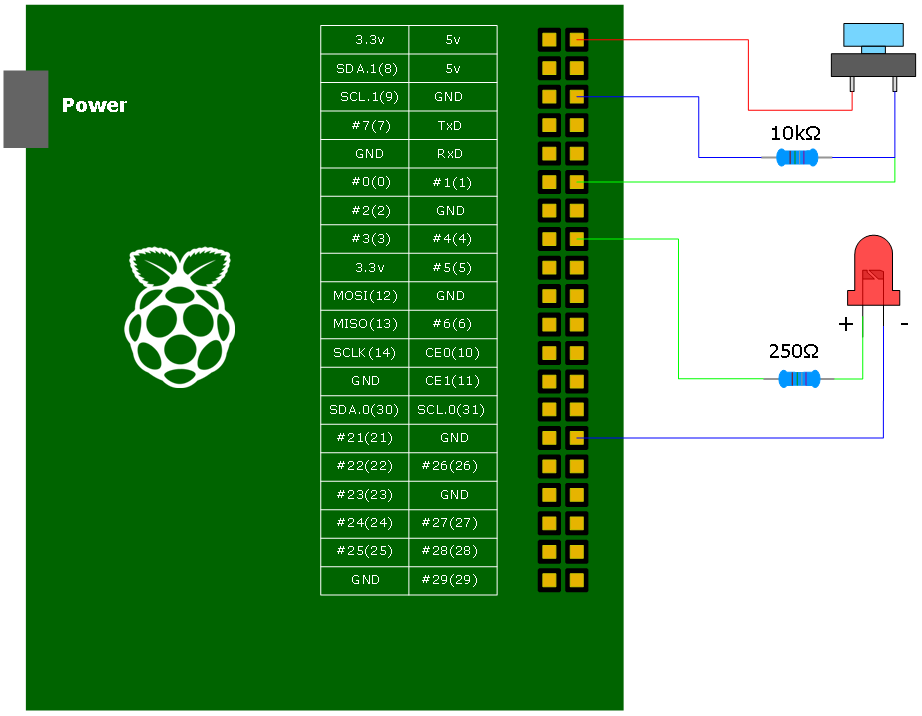
\includegraphics[width=1\textwidth]{./images/raspberry/ledbuttontest.png}
\caption{GPIO In/Out Test}
\label{fig:gpio_in_out}
\end{figure}
소스코드는 다음과 같다.
\begin{lstlisting}[style=termstylenumber, caption={Editing \texttt{/etc/fai/NFSROOT}}, label={list:nfsroot-file}]
#include <stdio.h>
#include <wiringPi.h>

#define LED 4
#define BUTTON 1

int main(void)
{
  if(wiringPiSetup() == -1)
    return 1;

  pinMode(LED, OUTPUT);
  pinMode(BUTTON, INPUT);

  digitalWrite(LED, 0);
  int input = 0;

  for(;;)
  {
    if(digitalRead(BUTTON))
      digitalWrite(LED, 1);
    else
      digitalWrite(LED, 0); 

    delay(100);
  }

  return 0;
}
\end{lstlisting}
컴파일 후 실행한다.
\begin{lstlisting}[style=termstyle]
pi@raspberrypi# gcc -o buttonTest buttonTest.c -lwiringPi
pi@raspberrypi# sudo ./buttonTest
\end{lstlisting}
버튼을 눌렀을 때 불이 들어오면 성공!
\subsection{PIR Motion Sensor}
PIR Motion 센서를 이용하여 동작을 감지해 보자. 그림\ref{fig:pir_test}과 같은 회로를 구성한다.
\begin{figure}[!htb]
\centering
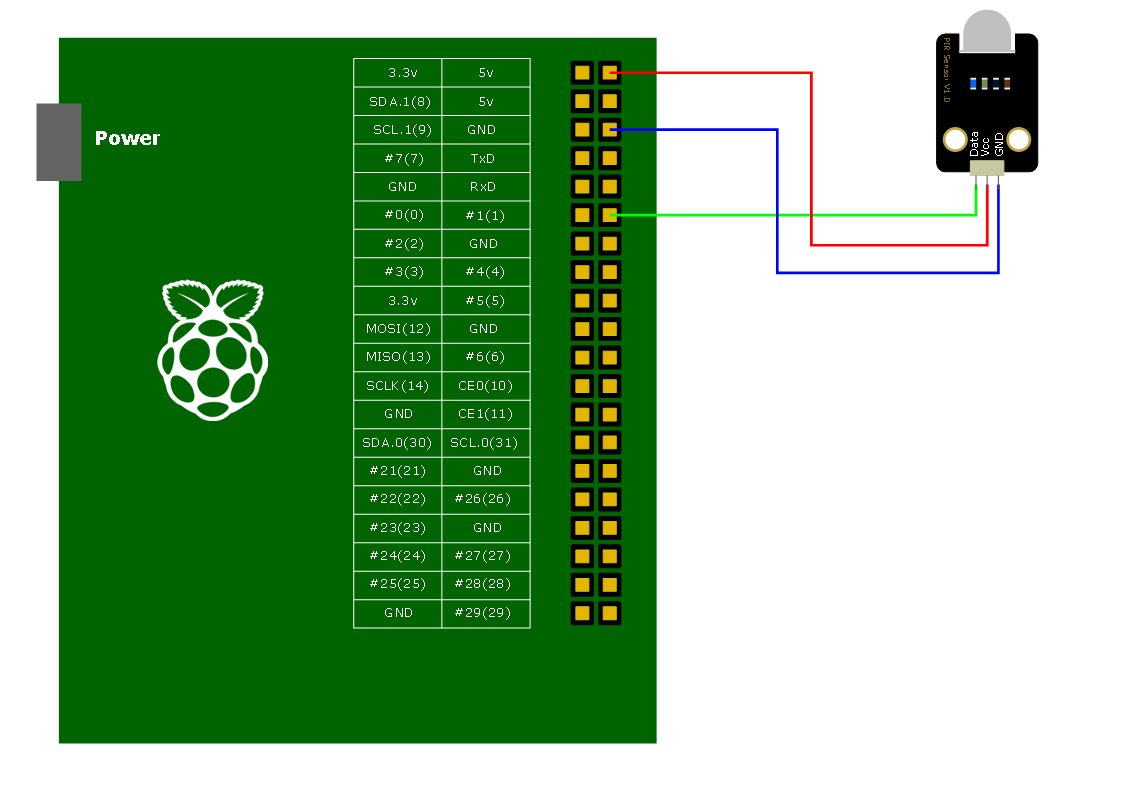
\includegraphics[width=1\textwidth]{./images/raspberry/pir_test.png}
\caption{PIR Motion Sensor Test}
\label{fig:pir_test}
\end{figure}
소스코드는 다음과 같다.
\begin{lstlisting}[style=termstylenumber, caption={Editing \texttt{/etc/fai/NFSROOT}}, label={list:nfsroot-file}]
#include <stdio.h>
#include <wiringPi.h>

#define PIR 1

int main(void)
{
  if(wiringPiSetup() == -1)
    return 1;

  pinMode(PIR, INPUT);

  int input = 0;

  for(;;)
  {
    if(digitalRead(PIR))
      printf("Motion Detected!\n");

    delay(100);
  }

  return 0;
}
\end{lstlisting}
컴파일 후 실행한다.
\begin{lstlisting}[style=termstyle]
pi@raspberrypi# gcc -o pir pir.c -lwiringPi
pi@raspberrypi# sudo ./pir
\end{lstlisting}
Motion이 감지되면 성공
\section{Humidity and Temperature Sensor}
\subsection{DHT11}
DHT11 센서를 이용하여 온도와 습도를 읽어 보자. 그림\ref{fig:dht11_test}와 같은 회로를 구성한다.
\begin{figure}[!htb]
\centering
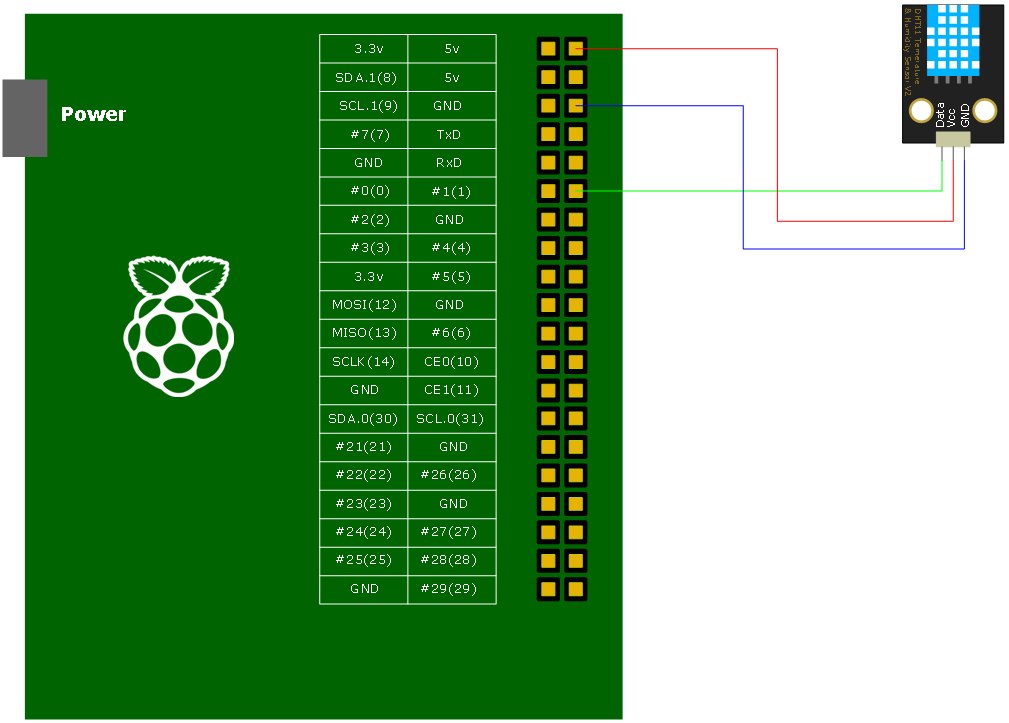
\includegraphics[width=1\textwidth]{./images/raspberry/dht11test.png}
\caption{DHT11 Sensor Test}
\label{fig:dht11_test}
\end{figure}
소스코드는 다음과 같다.
\begin{lstlisting}[style=termstylenumber, caption={Editing \texttt{/etc/fai/NFSROOT}}, label={list:nfsroot-file}]
#include <wiringPi.h>  
#include <stdio.h>  
#include <stdlib.h>  
#include <stdint.h> 

#define MAX_TIME 85  
#define DHT11PIN 1

int dht11_val[5]={0,0,0,0,0};  

void dht11_read_val()  
{  
uint8_t lststate=HIGH;  
  uint8_t counter=0;  
  uint8_t j=0,i;  

  for(i=0;i<5;i++)  
     dht11_val[i]=0;  

  pinMode(DHT11PIN,OUTPUT);  
  digitalWrite(DHT11PIN,LOW);  

  delay(18);  

  digitalWrite(DHT11PIN,HIGH);  

  delayMicroseconds(40);  

  pinMode(DHT11PIN,INPUT);  
  for(i=0;i<MAX_TIME;i++)  
  {  
    counter=0;  
    while(digitalRead(DHT11PIN)==lststate){  
      counter++;  
      delayMicroseconds(1);  
      if(counter==255)  
	break;  
    }  

    lststate=digitalRead(DHT11PIN);  

    if(counter==255)  
       break;  

    // top 3 transistions are ignored  
    if((i>=4)&&(i%2==0)){  
      dht11_val[j/8]<<=1;  
      if(counter>16)  
	dht11_val[j/8]|=1;  
      j++;  
    }  
  }  

  // verify cheksum and print the verified data  
  if((j>=40)&&(dht11_val[4]==((dht11_val[0]+dht11_val[1]+dht11_val[2]+dht11_val[3])& 0xFF)))  
  {  
    farenheit=dht11_val[2]*9./5.+32;  
    printf("H = %d.%d\nT = %d.%d\n",dht11_val[0],dht11_val[1],dht11_val[2],dht11_val[3]);  
  }  
  else  
    printf("Invalid Data!!\n");  
}  
  
int main(void)  
{  
  if(wiringPiSetup()==-1)  
    exit(1);  
  
  while(1)  
  {  
     dht11_read_val();  
       delay(1000);  
  }  
  
  return 0; 
}
\end{lstlisting}
컴파일 후 실행한다.
\begin{lstlisting}[style=termstyle]
pi@raspberrypi# gcc -o dht11 dht11.c -lwiringPi
pi@raspberrypi# sudo ./dht11
\end{lstlisting}
온습도 값이 출력되면 성공!
\subsection{DS1820}
DS1820 센서를 이용하여 온도를 읽어 보자.
\begin{figure}[!htb]
\centering
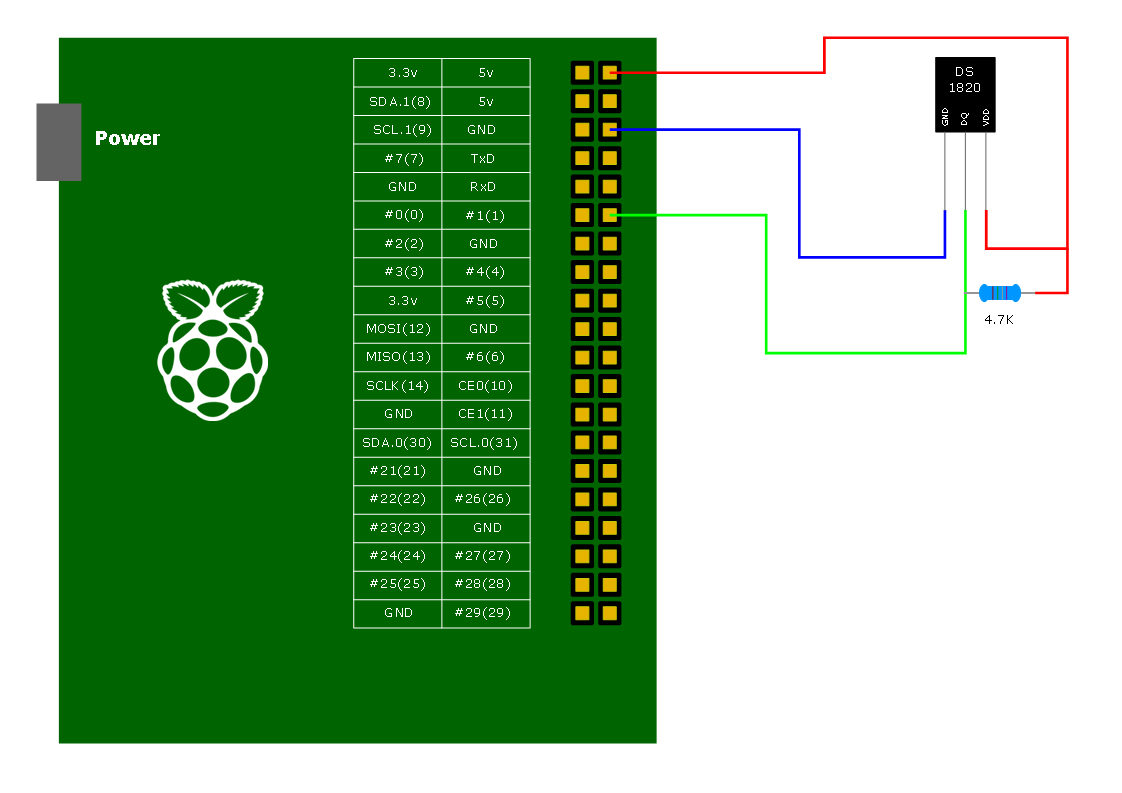
\includegraphics[width=1\textwidth]{./images/raspberry/ds1820_test.png}
\caption{DS1820 Temperature Sensor Test}
\label{fig:ds1820_test}
\end{figure}
소스코드는 다음과 같다.
\begin{lstlisting}[style=termstylenumber, caption={Editing \texttt{/etc/fai/NFSROOT}}, label={list:nfsroot-file}]
#include <stdio.h>
#include <string.h>
#include <stdlib.h>
#include <stdint.h>

#include <wiringPi.h>

#define PIN_NUM 1

float ds1820_read();
int onewire_reset();
void onewire_write(uint8_t data);
void onewire_write_bit(int bit);
uint8_t onewire_read();
int onewire_read_bit();
uint8_t crc_read();
uint8_t crc_cal(uint8_t crc, uint8_t data);

int main()
{
  if(wiringPiSetup() == -1)
    return 1;

  float temp = 0.0f;

  while(1)
  {
    temp = ds1820_read();
    printf("%.1f\n", temp);

   delay(1000);
  }
}
float ds1820_read()
{
  uint8_t busy = 1;

  onewire_reset();
  onewire_write(0xCC);
  onewire_write(0x44);

  delay(750);
  while(busy == 0)
  {
    busy = onewire_read();
    printf("busy: %d\n", busy);
  }

  onewire_reset();
  onewire_write(0xCC);
  onewire_write(0xBE);

  uint8_t lsb, msb, th, tl, reserved1, reserved2, count_remain, count_per_c, crc;
  float real_temp = 0.0f;
  signed char temp_read = 0;

  lsb = onewire_read();
  msb = onewire_read();
  th = onewire_read();
  tl = onewire_read();
  reserved1 = onewire_read();
  reserved2 = onewire_read();
  count_remain = onewire_read();
  count_per_c = onewire_read();
  crc = onewire_read();

  uint8_t data[] = {lsb, msb, th, tl, reserved1, reserved2, count_remain, count_per_c};

  onewire_reset();

  if(crc_read(data) == crc)
  {
    temp_read = (signed char)(lsb>>1);

    if(msb == 255)
      temp_read = temp_read | 0x80;

    real_temp = (float)temp_read + 0.85f - (float)count_remain/(float)count_per_c;
    real_temp = (int)(real_temp * 10) / 10.0f;
  }
  else
    printf("CRC Error  ");

  return real_temp;
}

int onewire_reset()
{
  int result;

  pinMode(PIN_NUM, OUTPUT);

  digitalWrite(PIN_NUM, LOW);
  delayMicroseconds(480);

  pinMode(PIN_NUM, INPUT);
  delayMicroseconds(70);

  result = digitalRead(PIN_NUM);

  delayMicroseconds(410);

  return result;
}

void onewire_write(uint8_t data)
{
  int loop;

  for(loop=0; loop<8; loop++)
  {
    onewire_write_bit(data & 0x01);

    data >>= 1;
  }
}
void onewire_write_bit(int bit)
{
  pinMode(PIN_NUM, OUTPUT);

  if(bit)
  {
    digitalWrite(PIN_NUM, LOW);
    delayMicroseconds(6);
    digitalWrite(PIN_NUM, HIGH);
    delayMicroseconds(64);
  }
  else
  {
    digitalWrite(PIN_NUM, LOW);
    delayMicroseconds(60);
    digitalWrite(PIN_NUM, HIGH);
    delayMicroseconds(10);
  }

}

uint8_t onewire_read()
{
  int loop, result=0;

  for(loop=0; loop<8; loop++)
  {
    result >>= 1;

    if(onewire_read_bit())
      result |= 0x80;
  }

  return result;
}

int onewire_read_bit()
{
  int result;

  pinMode(PIN_NUM, OUTPUT);

  digitalWrite(PIN_NUM, LOW);
  delayMicroseconds(6);

  pinMode(PIN_NUM, INPUT);
  delayMicroseconds(9);

  result = digitalRead(PIN_NUM) & 0x01;
  delayMicroseconds(55);

  return result;
}

uint8_t crc_read(uint8_t *data)
{
 uint8_t i, crc;

 crc = 0x00;

 for(i=0; i<8; i++)
  crc = crc_cal(crc, data[i]);

 return crc;
}

uint8_t crc_cal(uint8_t crc, uint8_t data)
{
  int j;
  for(j=0;j<8;j++) {
      if ((data & 0x01 ) ^ (crc & 0x01)) {
	  // DATA ^ LSB CRC = 1
	  crc = crc>>1;
	  // Set the MSB to 1
	  crc = crc | 0x80;
	  // Check bit 3
	  if (crc & 0x04) {
	      crc = crc & 0xFB; // Bit 3 is set, so clear it
	  } else {
	      crc = crc | 0x04; // Bit 3 is clear, so set it
	  }
	  // Check bit 4
	  if (crc & 0x08) {
	      crc = crc & 0xF7; // Bit 4 is set, so clear it
	  } else {
	      crc = crc | 0x08; // Bit 4 is clear, so set it
	  }
      } else {
	  // DATA ^ LSB CRC = 0
	  crc = crc>>1;
	  // clear MSB
	  crc = crc & 0x7F;
	  // No need to check bits, with DATA ^ LSB CRC = 0, they will remain unchanged
      }
      data = data>>1;
  }

  return crc;
}
\end{lstlisting}
컴파일 후 실행한다.
\begin{lstlisting}[style=termstyle]
pi@raspberrypi# gcc -o ds1820 ds1820.c -lwiringPi
pi@raspberrypi# sudo ./ds1820
\end{lstlisting}
온도 값이 출력되면 성공
\section{Dust Sensor}
\subsection{PM1001}
\section{Motor}
\subsection{L298 Dual H-Brdge}
Step Motor은 모터 종류에 따라 구동 방식이 다르다. 여기서는 Raspberry Pi와 
L298 Dual H-Bridge Motor Driver를 이용 하여 4 Wire 2Phase Step Motor를 작동하는 테스트를 하였다.
테스트는 다음 사이트를 참고 하였다.\\
http://www.geekonfire.com/wiki/index.php?title=Dual\_H-Bridge\_Motor\_Driver\\
http://www.raspberrypi.org/forums/viewtopic.php?f=49\&t=55580\\
사용된 하드웨어와 구성은 다음과 같다.
\begin{itemize}
\item Raspberry Pi Model B+
\item L298 Dual H-Bridge Motor Driver
\item 5V Power Supply
\item 스텝모터 (42HS40-1704A05)
\end{itemize}
\begin{figure}[!htb]
\centering
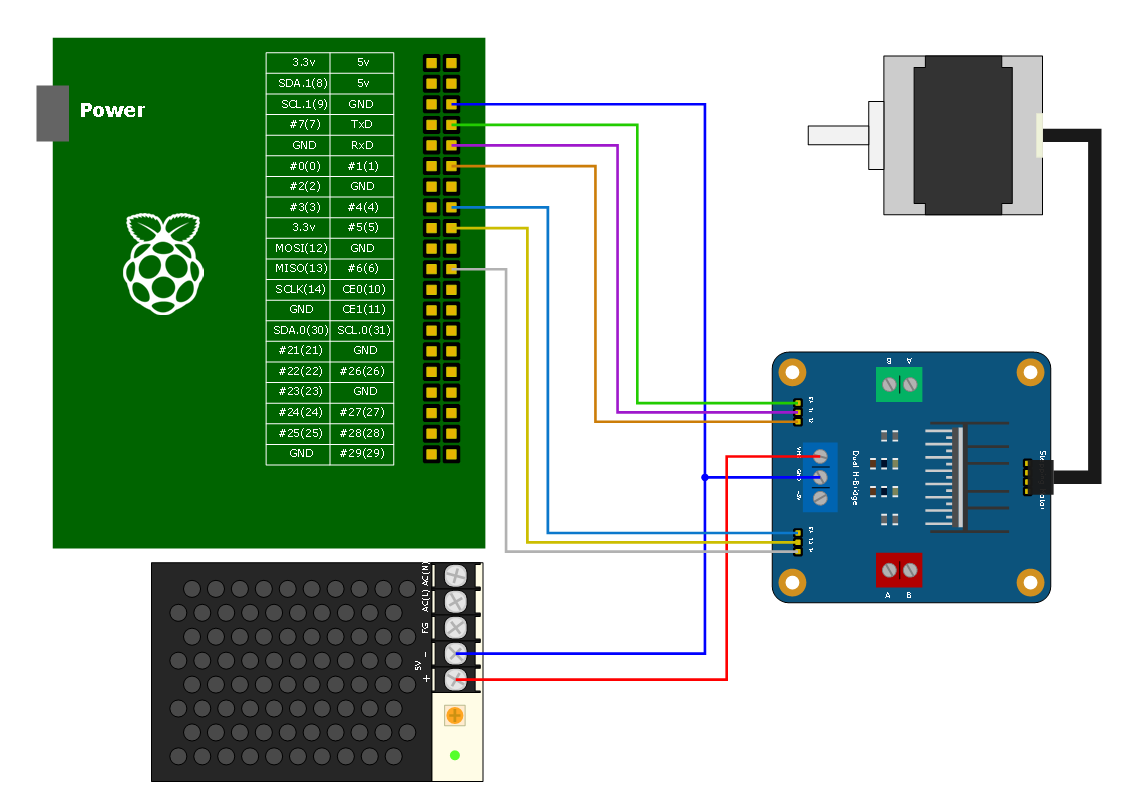
\includegraphics[width=1\textwidth]{./images/raspberry/L298Test.png}
\caption{2Phase Motor Test}
\label{fig:l298_test}
\end{figure}
코드 작성에 앞서 기본적인 작동 방식을 알아보자. 
4wire 2Phase Step Motor의 경우 다음과 같이 4개의 코일로 구성되어 있으며 2개의 코일이 같은 wire로 연결되다.
따라서 전류가 흐를 때 2개의 코일은 항상 반대 극성을 만들어 낸다.
\begin{figure}[!htb]
\centering
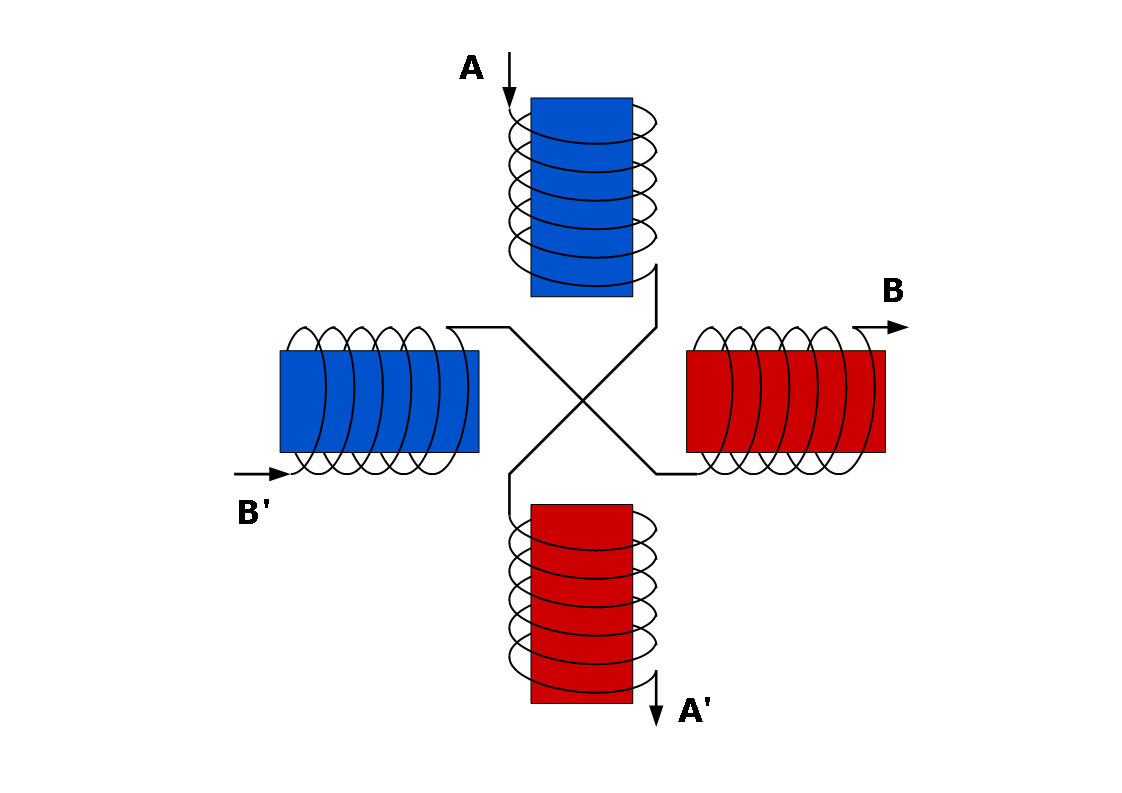
\includegraphics[width=1\textwidth]{./images/raspberry/stepMotor4wire2phase1.png}
\caption{2Phase Motor}
\label{fig:2phase_principle1}
\end{figure}
보통 스텝모터의 회전축은 영구자석으로 되어있으므로 다음과 같이 극성을 만들어 주면 모터가 회전하게 된다. 
그림에는 한 step당 90도 회전을 하지만 코일의 수를 늘이고 영구자석을 톱니모양으로 만들면 좀더 미세한 
각도로 회전한다. 일반적으로 많이 쓰이는 Step Motor의 Step 각도는 1.8도이다.
\begin{figure}[!htb]
\centering

\includegraphics[width=1\textwidth]{./images/raspberry/stepMotor4wire2phase2.png}
\caption{2Phase Motor Basic Principle}
\label{fig:2phase_principle2}
\end{figure}
참고로 실제 모터 구조와 작동 방법은 다음 그림에 가깝다.\\
그림 출처: http://www.orientalmotor.com/technology/articles/2phase-v-5phase.html
\begin{figure}[!htb]
\centering
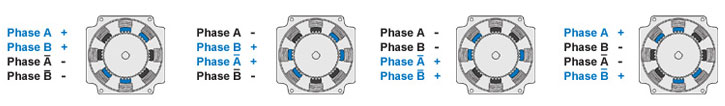
\includegraphics[width=1\textwidth]{./images/raspberry/2-ph-fullstep.jpg}
\caption{Real Motion}
\label{fig:2phase_principle3}
\end{figure}
실제로 위 그림과 같이 극성을 만들기 위해서는 코일에 전류를 순차적으로 흘러줘야 하는데 Motor Driver가 
외부 입력에 따라 모터에 전류를 공급한다. L298 Dual H-Bridge Motor Driver는 2개의 DC Motor 제어가 가능하다.
간단히 설명하면 총 6개의 입력신호 중 EA, IN1, IN2가 첫 번째 모터를, EB, IN3, IN4가 두 번째 모터를 
제어한다. EA, EB는 모터를 Enable 시키는 신호이며, IN1 ~ IN4는 모터의 전류 방향을 결정한다. 
즉, IN1과 IN2신호에 따라 전류 방향이 바뀌며 IN3와 IN4도 마찬가지 이다.
이걸 이용하면 4Wire 2Phase Step Motor에 순차적으로 전류를 흘러줄 수 있다. 
참고로 Step Motor의 경우 L298 Motor Driver에 있는 2개의 Motor 출력핀에 직접 연결해도 되고 Step Motor 
출력핀에 바로 연결해도 동일하게 동작한다.\\
이제 위 조건에 맞게 신호를 만드는 코드를 다음과 같이 작성한다.
\begin{lstlisting}[style=termstylenumber, caption={Editing \texttt{/etc/fai/NFSROOT}}, label={list:nfsroot-file}]
#include <stdio.h>
#include <wiringPi.h>

#define TRUE 1
#define FALSE 0
#define DELAY 1800

#define EA 15
#define EB 4
#define IN1 16
#define IN2 1
#define IN3 5
#define IN4 6

void setStep(int a, int b, int c, int d)
{
   digitalWrite(IN1, a);
   digitalWrite(IN2, b);
   digitalWrite(IN3, c);
   digitalWrite(IN4, d);
}

int main(void)
{
  if(wiringPiSetup() == -1)
  {
    printf("Init Error\n");
    return 1;
  }

  pinMode(EA, OUTPUT);
  pinMode(IN1, OUTPUT);
  pinMode(IN2, OUTPUT);
  pinMode(EB, OUTPUT);
  pinMode(IN3, OUTPUT);
  pinMode(IN4, OUTPUT);

  digitalWrite(EA, TRUE);
  digitalWrite(EB, TRUE);

  int i;
  int loop;

  for(;;)
  {
    for(i=0; i<500; i++)
    {
      setStep(1,0,1,0);
      delayMicroseconds(DELAY);
      setStep(0,1,1,0);
      delayMicroseconds(DELAY);
      setStep(0,1,0,1);
      delayMicroseconds(DELAY);
      setStep(1,0,0,1);
      delayMicroseconds(DELAY);
    }

    delay(1000);

    for(i=0; i<500; i++)
    {
      setStep(1,0,0,1);
      delayMicroseconds(DELAY);
      setStep(0,1,0,1);
      delayMicroseconds(DELAY);
      setStep(0,1,1,0);
      delayMicroseconds(DELAY);
      setStep(1,0,1,0);
      delayMicroseconds(DELAY);
    }

    delay(1000);

  }

  digitalWrite(EA, FALSE);
  digitalWrite(EB, FALSE);
\end{lstlisting}
위 코드에서 setStep함수는 IN신호를 만드는 함수로 총 4번의 Step이 1Cycle이 된다. 
1Step당 1.8도씩 회전하며 총 회전수는 반복문을 통해 제어 가능하다. 따라서 모터를 1회전 하고자 하면 
반복 횟수를 50(360 / 1.8 / 4)으로 하면 된다. 모터 속도는 DELAY시간에 따라 바뀌는데 시간이 너무 짧은 경우
회전하지 않는다. 모통 모터마다 최대 응답속도가 있으므로 그에 맞게 조절해야 한다. 테스트한 모터의 경우 
1.8ms(대략 167rpm)보다 짧은 경우 불규칙적인 회전을 보인다. Step신호를 반대로 주면 순서가 반대로 
작용하므로 모터 방향이 바뀐다. 모터의 방향은 Step순서를 반대로 하면 된다.
\subsection{MD5-DH14}
 여기서는 Raspberry Pi와 MD-DH14 Motor Driver를 이용하여 5Phase Pentagon방식의 Step Motor작동 테스트를 
하였다. 사용된 하드웨어와 구성은 다음과 같다.
\begin{figure}[!htb]
\centering
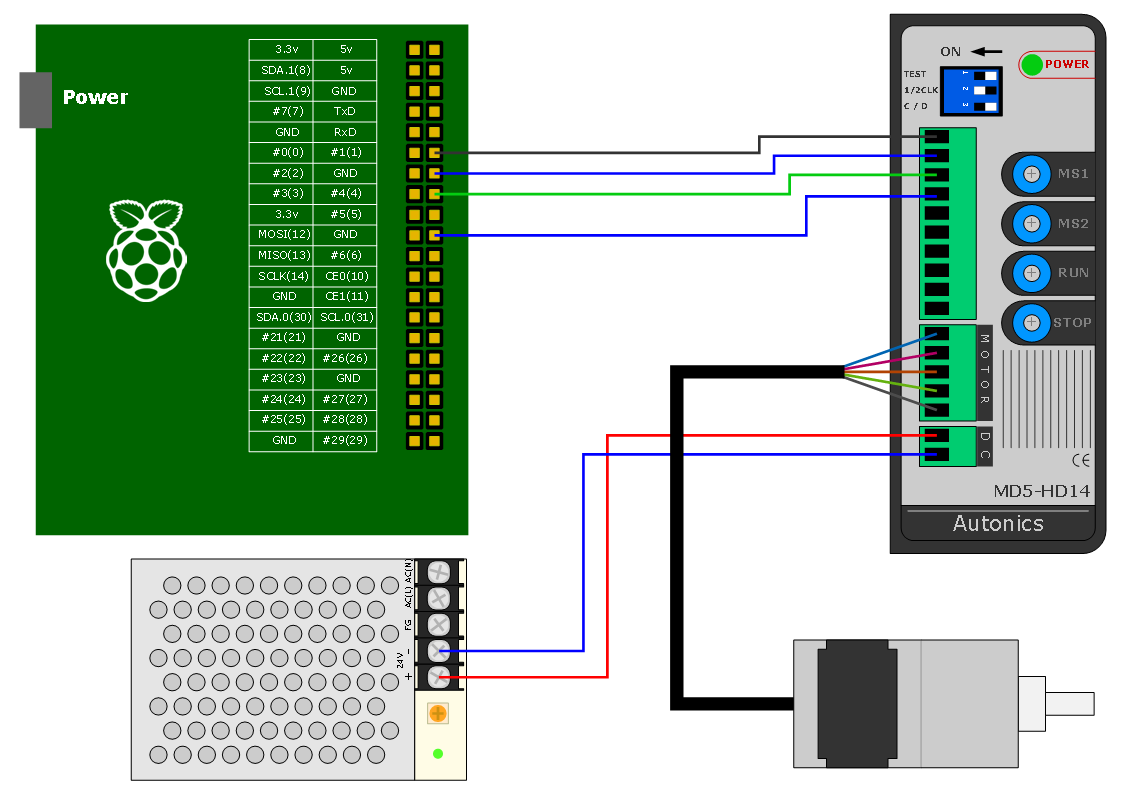
\includegraphics[width=1\textwidth]{./images/raspberry/md5dh14Test.png}
\caption{5Phase Motor Test}
\label{fig:5phase_test}
\end{figure}
\begin{itemize}
\item Raspberry Pi Model B+
\item MD5-HD14 Motor Driver
\item 24V Power Supply
\item 스텝모터 (A15K-S545-G10)
\end{itemize}
5Phase Step Motor는 작동 방식이 복잡한데 사실 Motor Driver가 알아서 구동시키므로 크게 고려할 필요는 없다.
참고로 대략적인 작동 방식은 다음 그림과 같다.\\
그림 출처: http://www.orientalmotor.com/technology/articles/2phase-v-5phase.html
\begin{figure}[!htb]
\centering
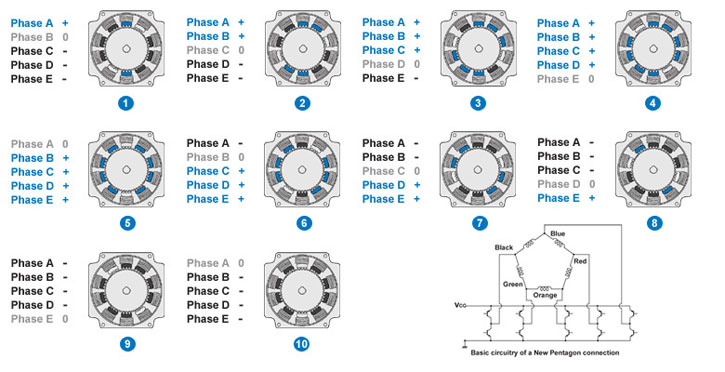
\includegraphics[width=1\textwidth]{./images/raspberry/5-ph-fullstep.jpg}
\caption{5Phase Motor Principle}
\label{fig:5phase_principle1}
\end{figure}
MD5-HD14 Motor Driver를 이용한 Step Motor 작동은 간단하다. 외부에서 Pulse 신호를 주면 Driver는 1Pulse당
1Step씩 Motor를 움직인다. 여기서 Step 각도는 연결된 Motor에 따라 다른데 테스트에 사용된 스텝모터는 
1Step당 0.072도씩 움직인다. 따라서 한바퀴를 돌리기 위해서는 5000Pulse가 필요하다. 
모터 방향을 바꾸는 방법은 2가지가 있는데 Driver에 있는 1/2 CLK 스위치에 따라 1Pulse방식과 2Pulse방식이 
있다. 1Pulse 방식은 CW 입력핀을 Pulse로 주고 CCW 입력핀에 따라 회전 방향을 결정하는 방식이다. 
2Pulse방식은 CW 입력핀과 CCW 입력핀에 각각 Pulse를 주는 방식이다. 이 경우 동시에 Pulse가 입력되면 
Motor가 작동 되지 않는다. 2Pulse 방식은 2개의 Pulse를 만들어야 하므로 테스트에는 1Pulse 방식을 
사용하였다. 이제 Motor 구동에 필요한 Pulse를 만드는 코드를 다음과 같이 작성한다. Pulse를 만드는 방법에 
대한 자세한 설명은 다음 페이지를 참고한다. 여기서는 GPIO를 이용하여 Pulse를 만들었다.
\begin{lstlisting}[style=termstylenumber, caption={Editing \texttt{/etc/fai/NFSROOT}}, label={list:nfsroot-file}]
#include <stdio.h>
#include <wiringPi.h>

#define PULSE 5000

int main(void)
{
  if(wiringPiSetup() == -1)
  {
    printf("Init Error\n");
    return 1;
  }

  pinMode(1, OUTPUT);
  pinMode(4, OUTPUT);

  int pulse;
  for(;;)
  {
    digitalWrite(4, 0);
    for(pulse=0; pulse<PULSE; pulse++)
    {
      digitalWrite(1, 1);
      delayMicroseconds(500);
      digitalWrite(1, 0);
      delayMicroseconds(500);
    }

    digitalWrite(4, 1);
    for(pulse=0; pulse<PULSE; pulse++)
    {
      digitalWrite(1, 1);
      delayMicroseconds(500);
      digitalWrite(1, 0);
      delayMicroseconds(500);
    }
  }
}

\end{lstlisting}
\chapter{EPICS Integration}
\section{GPIO}
Raspberry Pi는 40개의 입출력 Pin을 가지고 있는데(Model B의 경우 26개) 여기에서는 GPIO를 EPICS 에서 
사용하기 위한 방법과 테스트 과정에 대하여 설명하였다.\\
EPICS Application 폴더를 생성한다. 
\begin{lstlisting}[style=termstyle]
pi@ctrlpi3 cd ../epics/R3.14.12.4/siteApps
pi@ctrlpi3 ~/epics/R3.14.12.4/siteApps# mkdir gpio
pi@ctrlpi3 ~/epics/R3.14.12.4/siteApps# cd gpio
pi@ctrlpi3 ~/epics/R3.14.12.4/siteApps/gpio# makeBaseApp.pl -t ioc gpio
pi@ctrlpi3 ~/epics/R3.14.12.4/siteApps/gpio# makeBaseApp.pl -i -t ioc gpio

Using target architecture linux-arm (only one available)
The following applications are available:
    gpio
What application should the IOC(s) boot?
The default uses the IOC's name, even if not listed above.
Application name? gpio
pi@ctrlpi3 ~/epics/R3.14.12.4/siteApps/gpio# ls
conigure  gpioApp  iocBoot Makefile
\end{lstlisting}
gpioApp/src 폴더로 이동한 후 devGPIO.c 파일을 만들어 기본 코드를 작성한다.
\begin{lstlisting}[style=termstylenumber, caption={Editing \texttt{/etc/fai/NFSROOT}}, label={list:nfsroot-file}]
#include <stdio.h>
#include <string.h>
#include <stdlib.h>

#include <epicsExport.h>
#include <devSup.h>
#include <boRecord.h>
#include <biRecord.h>

#include <wiringPi.h>

static long bo_init_record(boRecord *pbo);
static long bi_init_record(biRecord *pbi);

static long write_bo(boRecord *pbo);
static long read_bi(biRecord *pbi);

static long bo_init_record(boRecord *pbo)
{
}

static long bi_init_record(biRecord *pbi)
{
}

static long write_bo(boRecord *pbo)
{
}

static long read_bi(biRecord *pbi)
{
}

struct
{
  long num;
  DEVSUPFUN     report;
  DEVSUPFUN     init;
  DEVSUPFUN     init_record;
  DEVSUPFUN     get_ioint_info;
  DEVSUPFUN     write_bo;
  DEVSUPFUN     special_linconv;
} devBoGpioAsync = {
  6,
  NULL,
  NULL,
  bo_init_record,
  NULL,
  write_bo,
  NULL
};

struct
{
  long num;
  DEVSUPFUN     report;
  DEVSUPFUN     init;
  DEVSUPFUN     init_record;
  DEVSUPFUN     get_ioint_info;
  DEVSUPFUN     read_bi;
  DEVSUPFUN     special_linconv;
} devBiGpioAsync = {
  6,
  NULL,
  NULL,
  bi_init_record,
  NULL,
  read_bi,
  NULL
};

epicsExportAddress(dset,devBoGpioAsync);
epicsExportAddress(dset,devBiGpioAsync);
\end{lstlisting}

\section{Humidity and Temperature Sensor}
Record는 출력을, biRecord는 입력을 위한 Record이며, 각각의 Record에 대한 초기화 함수와 GPIO를 
읽고 쓰기 위한 함수로 구성되어 있다. dset을 devBoGpioAsync와 devBiGpioAsync로 설정 하였으므로 
devGPIO.dbd 파일을 만들어 다음과 같이 작성한다. 
\begin{lstlisting}[style=termstyle]
device(bo, INST_IO, devBoGpioAsync, "GPIO")
device(bi, INST_IO, devBiGpioAsync, "GPIO")
\end{lstlisting}
기본 구조가 완성되었으면 실제 코드를 작성하도록 한다. 우선 초기화 함수를 다음과 같이 작성한다.
\begin{lstlisting}[style=termstylenumber, caption={Editing \texttt{/etc/fai/NFSROOT}}, label={list:nfsroot-file}]
static long bo_init_record(boRecord *pbo)
{
  struct Pin_Info *pin_info = malloc(sizeof(struct Pin_Info));

  if(wiringPiSetup() == -1)
    return 1;

  int pin_num = 0;
  pin_num = atoi(pbo->out.value.instio.string);

  pinMode(pin_num, OUTPUT);

  pin_info->pin_num = pin_num;

  pbo->dpvt = pin_info;

  return 0;
}

static long bi_init_record(biRecord *pbi)
{
  struct Pin_Info *pin_info = malloc(sizeof(struct Pin_Info));

  if(wiringPiSetup() == -1)
    return 1;

  int pin_num = 0;
  pin_num = atoi(pbi->inp.value.instio.string);

  pinMode(pin_num, INPUT);

  pin_info->pin_num = pin_num;

  pbi->dpvt = pin_info;

  return 0;
}
\end{lstlisting}
핀 번호를 저장하기 위한 구조체를 함수 선언 아래에 해준다.
\begin{lstlisting}[style=termstylenumber, caption={Editing \texttt{/etc/fai/NFSROOT}}, label={list:nfsroot-file}]
...
...
static long write_bo(boRecord *pbo);
static long read_bi(biRecord *pbi);

struct Pin_Info
{
  int pin_num;
}; 
\end{lstlisting}
bo와 bi초기화 코드는 거의 동일하며 차이는 bo의 경우 Link를 out에서, bi의 경우 Link를 inp에서 가져온다. 
또한 bo는 출력이므로 pinMode를 OUTPUT으로 설정하며 bi는 입력 모드인 INPUT로 설정한다.\\
초기화 함수가 완료되었으면 실제 값을 읽고 쓰는 함수를 작성한다. 우선 write\_bo 함수를 작성한다.
\begin{lstlisting}[style=termstylenumber, caption={Editing \texttt{/etc/fai/NFSROOT}}, label={list:nfsroot-file}]
static long write_bo(boRecord *pbo)
{
  struct Pin_Info *pin_info = pbo->dpvt;

  int pin = pin_info->pin_num;
  int val = pbo->rval;

  digitalWrite(pin, val);

  return 0;
}
\end{lstlisting}
GPIO 출력을 위해 wiringPi Library에 있는 digitalWrite 함수를 사용하는데 이 함수는 출력하고자 
하는 핀 번호와 출력값을 함수 인자로 받는다. 핀 번호는 앞서 dpvt 포인터에 저장된 구조체를 이용하여 
읽어온다. 출력 값은 boRecord 구조체 안에있는 rval변수로 부터 알 수 있다. 즉, 사용자가 다음과 같이 
값을 설정하면 그 값이 rval에 저장된다. 
\begin{lstlisting}[style=termstyle]
scwook@scwook:# caput out4 1
\end{lstlisting}
다음은 read\_bi 함수를 작성한다.
\begin{lstlisting}[style=termstylenumber, caption={Editing \texttt{/etc/fai/NFSROOT}}, label={list:nfsroot-file}]
static long read_bi(biRecord *pbi)
{
  struct Pin_Info *pin_info = pbi->dpvt;

  int pin = pin_info->pin_num;
  int val = digitalRead(pin);

  pbi->rval = val;

  return 0;
}
\end{lstlisting}
read\_bi함수는 write\_bo함수와 구조는 같으며 핀 값을 읽어들이는 digitalRead함수를 사용한다. 
이 함수는 핀 번호를 함수 인자로 받아 현재 핀 상태가 HIGH면 1, LOW면 0값을 리턴한다.\\
전체 코드는 다음과 같다.
\begin{lstlisting}[style=termstylenumber, caption={Editing \texttt{/etc/fai/NFSROOT}}, label={list:nfsroot-file}]
#include <stdio.h>
#include <string.h>
#include <stdlib.h>

#include <epicsExport.h>
#include <devSup.h>
#include <boRecord.h>
#include <biRecord.h>

#include <wiringPi.h>

static long bo_init_record(boRecord *pbo);
static long bi_init_record(biRecord *pbi);

static long write_bo(boRecord *pbo);
static long read_bi(biRecord *pbi);

struct Pin_Info
{
  int pin_num;
};

static long bo_init_record(boRecord *pbo)
{
  struct Pin_Info *pin_info = malloc(sizeof(struct Pin_Info));

  if(wiringPiSetup() == -1)
    return 1;

  int pin_num = 0;
  pin_num = atoi(pbo->out.value.instio.string);

  pinMode(pin_num, OUTPUT);

  pin_info->pin_num = pin_num;

  pbo->dpvt = pin_info;

  return 0;
}

static long bi_init_record(biRecord *pbi)
{
  struct Pin_Info *pin_info = malloc(sizeof(struct Pin_Info));

  if(wiringPiSetup() == -1)
    return 1;

  int pin_num = 0;
  pin_num = atoi(pbi->inp.value.instio.string);

  pinMode(pin_num, INPUT);

  pin_info->pin_num = pin_num;

  pbi->dpvt = pin_info;

  return 0;
}


static long write_bo(boRecord *pbo)
{
  struct Pin_Info *pin_info = pbo->dpvt;

  int pin = pin_info->pin_num;
  int val = pbo->rval;

  digitalWrite(pin, val);

  return 0;
}

static long read_bi(biRecord *pbi)
{
  struct Pin_Info *pin_info = pbi->dpvt;

  int pin = pin_info->pin_num;
  int val = digitalRead(pin);

  pbi->rval = val;

  return 0;
}

struct
{
  long num;
  DEVSUPFUN     report;
  DEVSUPFUN     init;
  DEVSUPFUN     init_record;
  DEVSUPFUN     get_ioint_info;
  DEVSUPFUN     write_bo;
  DEVSUPFUN     special_linconv;
} devBoGpioAsync = {
  6,
  NULL,
  NULL,
  bo_init_record,
  NULL,
  write_bo,
  NULL
};

struct
{
  long num;
  DEVSUPFUN     report;
  DEVSUPFUN     init;
  DEVSUPFUN     init_record;
  DEVSUPFUN     get_ioint_info;
  DEVSUPFUN     read_bi;
  DEVSUPFUN     special_linconv;
} devBiGpioAsync = {
  6,
  NULL,
  NULL,
  bi_init_record,
  NULL,
  read_bi,
  NULL
};

epicsExportAddress(dset,devBoGpioAsync);
epicsExportAddress(dset,devBiGpioAsync);
\end{lstlisting}
코드 작성이 완료되면 Makefile에 다음과 같이 추가한다.
\begin{lstlisting}[style=termstyle]
TOP=../..

include $(TOP)/configure/CONFIG

USR_INCLUDES += -I/home/pi/wiringPi/wiringPi
wiringPi_DIR += /home/pi/wiringPi/wiringPi /home/pi/wiringPi/devLib

#----------------------------------------
#  ADD MACRO DEFINITIONS AFTER THIS LINE
#=============================

#=============================
# Build the IOC application

PROD_IOC = gpio
# gpio.dbd will be created and installed
DBD += gpio.dbd

# gpio.dbd will be made up from these files:
gpio_DBD += base.dbd

# Include dbd files from all support applications:
#gpio_DBD += xxx.dbd
gpio_DBD += devGPIO.dbd

# Add all the support libraries needed by this IOC
#gpio_LIBS += xxx
gpio_LIBS += wiringPi

# gpio_registerRecordDeviceDriver.cpp derives from gpio.dbd
gpio_SRCS += gpio_registerRecordDeviceDriver.cpp
gpio_SRCS += devGPIO.c

# Build the main IOC entry point on workstation OSs.
gpio_SRCS_DEFAULT += gpioMain.cpp
gpio_SRCS_vxWorks += -nil-

# Add support from base/src/vxWorks if needed
#gpio_OBJS_vxWorks += $(EPICS_BASE_BIN)/vxComLibrary

# Finally link to the EPICS Base libraries
gpio_LIBS += $(EPICS_BASE_IOC_LIBS)

#===========================

include $(TOP)/configure/RULES
#----------------------------------------
#  ADD RULES AFTER THIS LINE
\end{lstlisting}
 이제 코드작성은 완료되었으므로 테스트를 위한 db파일을 만든다. gpioApp/Db 폴더로 이동한 후 gpio.db 
파일을 만든다. 
\begin{lstlisting}[style=termstyle]
record(bi, "inp1")
{
  field(DTYP, "GPIO")
  field(SCAN, "1 second")
  field(INP, "@1")
}

record(bo, "out4")
{
  field(DTYP, "GPIO")
  field(OUT, "@4")
}
\end{lstlisting}
gpio.db에서는 GPIO 1번을 입력으로 4번을 출력으로 설정했음을 알 수있다. Makefile에 db파일을 추가해 준다.
이제 컴파일을 하기 위해 gpio폴더로 이동한 후 make를 실행한다.
\begin{lstlisting}[style=termstyle]
pi@ctrlpi3 ~/epics/R3.14.12.4/siteApps/gpio# make
\end{lstlisting}
make가 완료되면 bin/linux-arm 폴더에 gpio 파일과 db 폴더에 gpio.db 파일이 만들어 진다.
이제 ioc를 실행시키기 위해 iocBoot/iocgpio 폴더로 이동 후 st.cmd파일에 gpio.db를 추가해 준다.
\begin{lstlisting}[style=termstyle]
#!../../bin/linux-arm/gpio

## You may have to change gpio to something else
## everywhere it appears in this file

< envPaths

cd ${TOP}

## Register all support components
dbLoadDatabase "dbd/gpio.dbd"
gpio_registerRecordDeviceDriver pdbbase

## Load record instances
#dbLoadTemplate "db/userHost.substitutions"
#dbLoadRecords "db/dbSubExample.db", "user=piHost"
dbLoadRecords "db/gpio.db"

## Set this to see messages from mySub
#var mySubDebug 1

## Run this to trace the stages of iocInit
#traceIocInit

cd ${TOP}/iocBoot/${IOC}
iocInit

## Start any sequence programs
#seq sncExample, "user=piHost"
\end{lstlisting}
마지막으로 st.cmd파일을 실행파일로 변경한 후 실행시킨다.
\begin{lstlisting}[style=termstyle]
pi@ctrlpi3 ~/epics/R3.14.12.4/siteApps/gpio/iocBoot/iocdht11 $ chmod 755 st.cmd
pi@ctrlpi3 ~/epics/R3.14.12.4/siteApps/gpio/iocBoot/iocdht11 $ sudo ./st.cmd
\end{lstlisting}
out4 출력값을 1로 했을 때 LED에 불이오면 성공!
\begin{lstlisting}[style=termstyle]
epics> dbpf out4 1
\end{lstlisting}
버튼을 누른 상태에서 inp1 값이 1이면 성공!
\begin{lstlisting}[style=termstyle]
epics> dbpr inp1
ASG:                DESC:               DISA: 0             DISP: 0             
DISV: 1             NAME: gpio:inp1     RVAL: 0             SEVR: NO_ALARM      
STAT: NO_ALARM      SVAL: 0             TPRO: 0             VAL: 1
\end{lstlisting}
\subsection{Library}
지금까지 만든 코드를 Library로 만들어 보자.
siteLibs 폴더로 이동한 후 raspGPIOLib 폴더를 하나 만든다.
\begin{lstlisting}[style=termstyle]
pi@ctrlpi3 ~/epics/R3.14.12.4/siteLibs $ mkdir raspGPIOLib
pi@ctrlpi3 ~/epics/R3.14.12.4/siteLibs $ cd raspGPIOLibs
pi@ctrlpi3 ~/epics/R3.14.12.4/siteLibs/raspGPIOLibs $
\end{lstlisting}
rsapGPIOLib 폴더안에 Db, src폴더를 만들고 Makefile을 생성한 후 다음과 같이 작성한다.
\begin{lstlisting}[style=termstyle]
TOP = ..
include $(TOP)/configure/CONFIG
DIRS := $(DIRS) $(filter-out $(DIRS), $(wildcard *src*))
DIRS := $(DIRS) $(filter-out $(DIRS), $(wildcard *Src*))
DIRS := $(DIRS) $(filter-out $(DIRS), $(wildcard *db*))
DIRS := $(DIRS) $(filter-out $(DIRS), $(wildcard *Db*))
include $(TOP)/configure/RULES_DIRS
\end{lstlisting}
src 폴더로 이동 후 지금까지 만든 devGPIO.c와 devGPIO.dbd 파일을 복사한다.
\begin{lstlisting}[style=termstyle]
pi@ctrlpi3 ~/epics/R3.14.12.4/siteLibs/raspGPIOLibs/src $ cp /home/pi/epics/R3.14.12.4/siteApps/gpio/gpioApp/src/devGPIO.c ./
pi@ctrlpi3 ~/epics/R3.14.12.4/siteLibs/raspGPIOLibs/src $ cp /home/pi/epics/R3.14.12.4/siteApps/gpio/gpioApp/src/devGPIO.dbd ./
\end{lstlisting}
Makefile 만들고 다음과 같이 작성한다.
\begin{lstlisting}[style=termstyle]
TOP = ../..
include $(TOP)/configure/CONFIG

LIBRARY_IOC += raspGPIO
DBD         += devGPIO.dbd
raspGPIO_SRCS += devGPIO.c

include $(TOP)/configure/RULES
\end{lstlisting}
 src 폴더안에서 make를 실행한다. make가 완료되면 siteLibs/lib/linux-arm 폴더안에 libraspGPIO.so 파일이 
만들어 진다. Library에 대한 db파일 제공을 위해 raspGPIOLibs/Db폴더로 이동한 후 다음과 같은 
gpio.db파일만든다.
\begin{lstlisting}[style=termstyle]
record(bi, "inp1")
{
  field(DTYP, "GPIO")
  field(SCAN, "1 second")
  field(INP, "@1")
}

record(bo, "out4")
{
  field(DTYP, "GPIO")
  field(OUT, "@4")
}
\end{lstlisting}
Makefile을 만들어 다음과 같이 작성한다.
\begin{lstlisting}[style=termstyle]
TOP =../..
include $(TOP)/configure/CONFIG
DB += gpio.db
include $(TOP)/configure/RULES
\end{lstlisting}
make를 실행하면 siteLibs/db 폴더안에 gpio.db파일이 생성된다.
Library를 이용한 GPIO 테스트는 EPICS Application에 있는 GPIO Input/Output Test with LED and 
Button을 참고하기 바란다.
\section{Dust Sensor}
PM1001 먼지 센서는 1um이상의 먼지를 감지하여 수량PCS/L값 으로 출력해 주는 센서이다. 센서에 대한 자세한 
사양은 다음 홈페이지를 참고하기 바란다.\\
http://www.diwellshop.com/product/detail.html?product\_no=172\&cate\_no=36\&display\_group=1\\
테스트에 사용된 하드웨어 구성은 다음과 같다.
\begin{figure}[!htb]
\centering
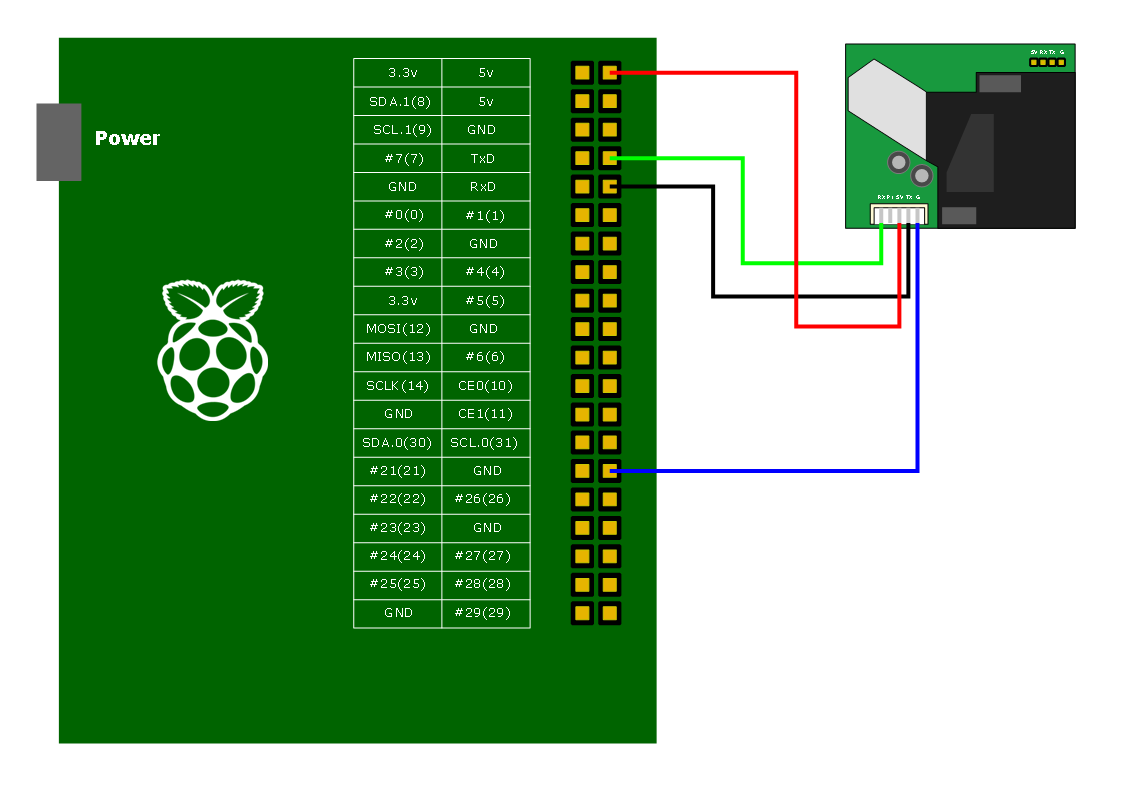
\includegraphics[width=1\textwidth]{./images/epics/PM1001Test.png}
\caption{PM1001 Dust Sensor Test}
\label{fig:pm1001_epics_test}
\end{figure}
 PM1001의 경우 UART 통신을 통해 데이터를 전송하므로 Raspberry Pi의 UART 포트와 연결이 가능하다. 
참고로 UART(Universal asynchronous receiver/transmitter)는 일반적으로 RS-232와 같은 시리얼 통신을 
5V Level의 TTL신호로 전송한다. 따라서 Raspberry Pi나 Arduino와 같이 UART를 지원하는 보드에서는 바로 
연결하여 사용이 가능하다. 여기서 주의할 사항은 PC의 경우 Serial 통신의 전압 Level이 -12 ~ 12v이므로 
센서와 바로 연결해서는 안되며 MAX232와 같은 Level Convert를 사용하여 전압 Level을 맞춰야 한다. 여기서는 
Raspberry Pi에 바로 연결하여 테스트 하였으므로 별도의 Convert를 사용하지 않았다.\\
Raspberry Pi에서 UART는 기본적으로 콘솔출력용으로 지정되어 있다. 
따라서 일반적인 목적으로 사용하기 위해서는 /boot/cmdline.txt와 /etc/inittab 파일을 수정해야 한다.\\
/boot/cmdline.txt 파일을 열어 "console=ttyAMA0,115200" 부분을 삭제 한다.
\begin{lstlisting}[style=termstyle]
dwc_otg.lpm_enable=0 console=ttyAMA0,115200 console=tty1 root=/dev/mmcblk0p2 rootfstype=ext4 elevator=de$
\end{lstlisting}
/etc/inittab 파일을 열어 마지막 라인에 있는 "T0:23:respawn:/sbin/getty -L ttyAMA0 115200 vt100" 
앞에 '\#'을 넣어 주석 처리한다
\begin{lstlisting}[style=termstyle]
# /etc/inittab: init(8) configuration.
# $Id: inittab,v 1.91 2002/01/25 13:35:21 miquels Exp $

# The default runlevel.
id:2:initdefault:

# Boot-time system configuration/initialization script.
# This is run first except when booting in emergency (-b) mode.
si::sysinit:/etc/init.d/rcS

# What to do in single-user mode.
~~:S:wait:/sbin/sulogin

# /etc/init.d executes the S and K scripts upon change
# of runlevel.
#
# Runlevel 0 is halt.
# Runlevel 1 is single-user.
# Runlevels 2-5 are multi-user.
# Runlevel 6 is reboot.

l0:0:wait:/etc/init.d/rc 0
l1:1:wait:/etc/init.d/rc 1
l2:2:wait:/etc/init.d/rc 2
l3:3:wait:/etc/init.d/rc 3
l4:4:wait:/etc/init.d/rc 4
l5:5:wait:/etc/init.d/rc 5
l6:6:wait:/etc/init.d/rc 6
# Normally not reached, but fallthrough in case of emergency.
z6:6:respawn:/sbin/sulogin

# What to do when CTRL-ALT-DEL is pressed.
ca:12345:ctrlaltdel:/sbin/shutdown -t1 -a -r now

# Action on special keypress (ALT-UpArrow).
#kb::kbrequest:/bin/echo "Keyboard Request--edit /etc/inittab to let this work."

# What to do when the power fails/returns.
pf::powerwait:/etc/init.d/powerfail start
pn::powerfailnow:/etc/init.d/powerfail now
po::powerokwait:/etc/init.d/powerfail stop

# /sbin/getty invocations for the runlevels.
#
# The "id" field MUST be the same as the last
# characters of the device (after "tty").
#
# Format:
#  <id>:<runlevels>:<action>:<process>
#
# Note that on most Debian systems tty7 is used by the X Window System,
# so if you want to add more getty's go ahead but skip tty7 if you run X.
#
1:2345:respawn:/sbin/getty --noclear 38400 tty1
2:23:respawn:/sbin/getty 38400 tty2
3:23:respawn:/sbin/getty 38400 tty3
4:23:respawn:/sbin/getty 38400 tty4
5:23:respawn:/sbin/getty 38400 tty5
6:23:respawn:/sbin/getty 38400 tty6

# Example how to put a getty on a serial line (for a terminal)
#
#T0:23:respawn:/sbin/getty -L ttyS0 9600 vt100
#T1:23:respawn:/sbin/getty -L ttyS1 9600 vt100

# Example how to put a getty on a modem line.
#
#T3:23:respawn:/sbin/mgetty -x0 -s 57600 ttyS3


#Spawn a getty on Raspberry Pi serial line
#T0:23:respawn:/sbin/getty -L ttyAMA0 115200 vt100
\end{lstlisting}
설정을 마쳤으면 재부팅 한다. 
\begin{lstlisting}[style=termstyle]
pi@raspberrypi~$ sudo reboot
\end{lstlisting}
재부팅이 완료되면 UART를 사용할 수 있다. 참고로 Raspberry Pi에서는 UART device는 /etc/ttyAMA0에 할당되어
있다 PM1001 센서는 시리얼 통신을 사용하므로 EPICS Asyn과 StreamDevice Library를 설치한다.
우선 stieLibs로 이동한다. siteLibs가 없다면 svn에서 내려 받는다.
\begin{lstlisting}[style=termstyle]
pi@raspberrypi ~/epics/R3.14.12.4 $ svn co svn://10.1.5.14/raon/trunk/siteLibs
\end{lstlisting}
siteLibs안에 있는 asyn-4-21과 stream2-6 폴더로 이동한 후 make를 실행한다.
\begin{lstlisting}[style=termstyle]
pi@raspberrypi ~/epics/R3.14.12.4 $ cd siteLibs/asyn-4-21
pi@raspberrypi ~/epics/R3.14.12.4/siteLibs/asyn-4-21 $ make
pi@raspberrypi ~/epics/R3.14.12.4/siteLibs/asyn-4-21 $ cd ../stream-2-6
pi@raspberrypi ~/epics/R3.14.12.4/siteLibs/stream-2-6 $ make
\end{lstlisting}
make가 완료되면 siteLibs/lib/linux-arm 폴더에 libasyn.so와 libstream.so파일이 생성된다.
이제 siteApps폴더로 이동한 후 App폴더를 만든다. siteApps폴더가 없다면 svn으로 부터 내려 받는다.
\begin{lstlisting}[style=termstyle]
pi@raspberrypi ~/epics/R3.14.12.4 $ svn co svn://10.1.5.14/raon/trunk/siteApps
\end{lstlisting}
siteApps 폴더안에 pm1001폴더를 생성한 다음 기본 ioc구조를 만든다.
\begin{lstlisting}[style=termstyle]
pi@raspberrypi ~/epics/R3.14.12.4 $ cd siteApps
pi@raspberrypi ~/epics/R3.14.12.4/siteApps $ mkdir pm1001
pi@raspberrypi ~/epics/R3.14.12.4/siteApps $ cd pm1001
pi@raspberrypi ~/epics/R3.14.12.4/siteApps/pm1001 $ makeBaseApp.pl -t ioc pm1001
pi@raspberrypi ~/epics/R3.14.12.4/siteApps/pm1001 $ makeBaseApp.pl -i -t ioc pm1001
Using target architecture linux-arm (only one available)
The following applications are available:
    pm1001
What application should the IOC(s) boot?
The default uses the IOC's name, even if not listed above.
Application name? pm1001
\end{lstlisting}
pm1001/configure/RELEASE 파일에 asyn과 stream Library위치를 추가해 준다.
\begin{lstlisting}[style=termstyle]
# RELEASE - Location of external support modules
#
# IF YOU MAKE ANY CHANGES to this file you must subsequently
# do a "gnumake rebuild" in this application's top level
# directory.
#
# The build process does not check dependencies against files
# that are outside this application, thus you should do a
# "gnumake rebuild" in the top level directory after EPICS_BASE
# or any other external module pointed to below is rebuilt.
#
# Host- or target-specific settings can be given in files named
#  RELEASE.$(EPICS_HOST_ARCH).Common
#  RELEASE.Common.$(T_A)
#  RELEASE.$(EPICS_HOST_ARCH).$(T_A)
#
# This file should ONLY define paths to other support modules,
# or include statements that pull in similar RELEASE files.
# Build settings that are NOT module paths should appear in a
# CONFIG_SITE file.

TEMPLATE_TOP=$(EPICS_BASE)/templates/makeBaseApp/top

# If using the sequencer, point SNCSEQ at its top directory:
#SNCSEQ=$(EPICS_BASE)/../modules/soft/seq

# EPICS_BASE usually appears last so other apps can override stuff:
EPICS_BASE=/home/pi/epics/R3.14.12.4/base

# Set RULES here if you want to take build rules from somewhere
# other than EPICS_BASE:
#RULES=/path/to/epics/support/module/rules/x-y

ASYN=$(EPICS_PATH)/siteLibs
STREAM=$(EPICS_PATH)/siteLibs
\end{lstlisting}
pm1001App/src 폴더로 이동하면 pm1001Main.cpp와 Makefile이 있다. Makefile에 다음 코드를 추가한다.
\begin{lstlisting}[style=termstyle]
TOP=../..

include $(TOP)/configure/CONFIG
#----------------------------------------
#  ADD MACRO DEFINITIONS AFTER THIS LINE
#=============================

#=============================
# Build the IOC application

PROD_IOC = pm1001
# pm1001.dbd will be created and installed
DBD += pm1001.dbd

# pm1001.dbd will be made up from these files:
pm1001_DBD += base.dbd

# Include dbd files from all support applications:
#pm1001_DBD += xxx.dbd

pm1001_DBD += stream.dbd
pm1001_DBD += drvAsynSerialPort.dbd

# Add all the support libraries needed by this IOC
#pm1001_LIBS += xxx

pm1001_LIBS += stream
pm1001_LIBS += asyn

# pm1001_registerRecordDeviceDriver.cpp derives from pm1001.dbd
pm1001_SRCS += pm1001_registerRecordDeviceDriver.cpp

# Build the main IOC entry point on workstation OSs.
pm1001_SRCS_DEFAULT += pm1001Main.cpp
pm1001_SRCS_vxWorks += -nil-

# Add support from base/src/vxWorks if needed
#pm1001_OBJS_vxWorks += $(EPICS_BASE_BIN)/vxComLibrary

# Finally link to the EPICS Base libraries
pm1001_LIBS += $(EPICS_BASE_IOC_LIBS)

#===========================

include $(TOP)/configure/RULES
#----------------------------------------
#  ADD RULES AFTER THIS LINE
\end{lstlisting}
이제 필요한 Library는 사용준비가 되었으므로 db와 proto 파일을 만들도록 한다. 
pm1001App/Db 폴더로 이동하여 pm1001.db 파일을 만들고 Makefile에 추가해 준다. 
\begin{lstlisting}[style=termstyle]
record(ai,"SS:DUST")
{
  field(DTYP, "stream")
  field(INP, "@sensor.proto get_dust UART")
  field(SCAN, "1 second")
}
\end{lstlisting}
\begin{lstlisting}[style=termstyle]
TOP=../..
include $(TOP)/configure/CONFIG
#----------------------------------------
#  ADD MACRO DEFINITIONS AFTER THIS LINE

#----------------------------------------------------
#  Optimization of db files using dbst (DEFAULT: NO)
#DB_OPT = YES

#----------------------------------------------------
# Create and install (or just install) into /db
# databases, templates, substitutions like this
#DB += xxx.db
DB += pm1001.db

#----------------------------------------------------
# If .db template is not named *.template add
# _template = 

include $(TOP)/configure/RULES
#----------------------------------------
#  ADD RULES AFTER THIS LINE
\end{lstlisting}
proto 파일을 만들기 앞서 pm1001 센서의 통신 명령어를 알아야 한다. 메뉴얼을 참고하면 통신 명령어가 다음과
같음을 알 수 있다.

        SEND: [IP] [LB] [CMD] [DF] [CS]

        RESPONSE: [ACK] [LB] [CMD] [DF] [CS]

여기서 각 명령에 대한 의미는 다음과 같다.

        [IP]: address(fixed as 0x11)
        [LB]: byte length followed does not include CS
        [CMD]: command
        [DF]: parameter items with command, optional
        [CS]: CS = -(IP + LB + CMD + DF)
        [ACK] 0x16 right command

예를 들어 PM1001로 부터 먼지 값을 읽는 명령어는 다음과 같다.
        SEND: 0X11, 0X01, 0X01, 0XED
        RESPONSE: 0x16, 0x0D, 0x01, 4BytePM값, 4BytePM값, 4BytePM값, [CS]
여기서 PM값은 4Byte(DF0, DF1, DF2, DF3)로 구성된 먼지 데이터 값으로 측정 값은 다음과 같다.
        Measured value = DF0 * 256 * 256 * 256 + DF1 * 256 * 256 + DF2 * 256 + DF3
참고로 값은 값이 3번 반복해서 출력되므로 첫 번째 값만 읽으면 된다.
이제 proto 파일을 만들기 위해 pm1001에서 proto폴더를 하나 만든 후 pm1001.proto 파일을 다음과 같이 작성한다.
\begin{lstlisting}[style=termstyle]
pi@raspberrypi ~/epics/R3.14.12.4/siteApps/pm1001 $ mkdir proto
pi@raspberrypi ~/epics/R3.14.12.4/siteApps/pm1001 $ cd proto
\end{lstlisting}
\begin{lstlisting}[style=termstyle]
get_dust{
	out "\x11\x01\x01\xED";
	in "%*3r%4r%*4r%*4r%*1r";
}
\end{lstlisting}
get\_dust 함수는 out을 통해 먼지 값을 읽어오는 명령을 전송한다. pm1001 센서는 응답 값으로 총 16byte의 
값을 리턴하는데 이 중 먼지 데이터는 처음 3byte 이후 4byte 씩 3번 반복되므로 첫 4byte만 저장하고 
checksum을 포함한 나머지 byte는 무시한다. 참고로 읽고자 하는 값을 무시 하고 싶을 때는 '*'를 앞에다
붙이면 된다. 여기에서는 4byte를 읽으므로 앞서 말한 Measured value를 계산하기 위해 256을 곱하지 않아도 
된다. 만약 DF0 ~ DF3을 따로 읽고자 하면 다음과 같이 1byte씩 읽으면 된다. 
\begin{lstlisting}[style=termstyle]
get_d0{
	out "\x11\x01\x01\xED";
	in "%*3r%1r%*3r%*4r%*4r%*1r";
}

get_d1{
	out "\x11\x01\x01\xED";
	in "%*3r%*1r%1r%*2r%*4r%*4r%*1r";
}

get_d2{
	out "\x11\x01\x01\xED";
	in "%*3r%*2r%1r%*1r%*4r%*4r%*1r";
}

get_d3{
	out "\x11\x01\x01\xED";
	in "%*3r%*3r%1r%*4r%*4r%*1r";
}
\end{lstlisting}
이제 pm1001폴더로 이동하여 make를 실행하자
\begin{lstlisting}[style=termstyle]
pi@raspberrypi ~/epics/R3.14.12.4/siteApps/pm1001 $ make
\end{lstlisting}
ioc를 실행하기 위해 iocBoot/iocpm1001로 이동 후 st.cmd 파일에 다음과 같이 추가 한다.
\begin{lstlisting}[style=termstyle]
#!../../bin/linux-arm/pm1001

## You may have to change pm1001 to something else
## everywhere it appears in this file

< envPaths

cd ${TOP}

epicsEnvSet "STREAM_PROTOCOL_PATH" "../../proto"

## Register all support components
dbLoadDatabase "dbd/pm1001.dbd"
pm1001_registerRecordDeviceDriver pdbbase

drvAsynSerialPortConfigure "UART" "/dev/ttyAMA0"

asynSetOption("UART", 0, "baud", "9600")
asynSetOption("UART", 0, "bits", "8")
asynSetOption("UART", 0, "parity", "none")

## Load record instances
#dbLoadRecords("db/xxx.db","user=piHost")
dbLoadRecords("db/pm1001.db")

cd ${TOP}/iocBoot/${IOC}
iocInit

## Start any sequence programs
#seq sncxxx,"user=piHost"
\end{lstlisting}
st.cmd를 실행파일로 변경한 후 실행한다.
\begin{lstlisting}[style=termstyle]
pi@raspberrypi ~/epics/R3.14.12.4/siteApps/pm1001/iocBoot/iocpm1001 $ chmod 755 st.cmd
pi@raspberrypi ~/epics/R3.14.12.4/siteApps/pm1001/iocBoot/iocpm1001 $ sudo ./st.cmd
#!../../bin/linux-arm/pm1001
## You may have to change pm1001 to something else
## everywhere it appears in this file
< envPaths
epicsEnvSet("ARCH","linux-arm")
epicsEnvSet("IOC","iocpm1001")
epicsEnvSet("TOP","/home/pi/epics/R3.14.12.4/siteApps/pm1001")
epicsEnvSet("EPICS_BASE","/home/pi/epics/R3.14.12.4/base")
cd /home/pi/epics/R3.14.12.4/siteApps/pm1001
epicsEnvSet "STREAM_PROTOCOL_PATH" "../../proto"
## Register all support components
dbLoadDatabase "dbd/pm1001.dbd"
pm1001_registerRecordDeviceDriver pdbbase
drvAsynSerialPortConfigure "UART" "/dev/ttyAMA0"
asynSetOption("UART", 0, "baud", "9600")
asynSetOption("UART", 0, "bits", "8")
asynSetOption("UART", 0, "parity", "none")
## Load record instances
#dbLoadRecords("db/xxx.db","user=piHost")
dbLoadRecords("db/sensor.db")
cd /home/pi/epics/R3.14.12.4/siteApps/pm1001/iocBoot/iocpm1001
iocInit
Starting iocInit
############################################################################
## EPICS R3.14.12.4 $Date: Mon 2013-12-16 15:51:45 -0600$
## EPICS Base built Oct  4 2014
############################################################################
iocRun: All initialization complete
## Start any sequence programs
#seq sncxxx,"user=piHost"
\end{lstlisting}
먼지 값이 읽어지면 끝!
\begin{lstlisting}[style=termstyle]
epics> dbpr SS:DUST
ASG:                DESC:               DISA: 0             DISP: 0             
DISV: 1             NAME: SS:DUST       RVAL: 673           SEVR: NO_ALARM      
STAT: NO_ALARM      SVAL: 0             TPRO: 0             VAL: 673
\end{lstlisting}
참고로 pm1001 센서는 먼지 값을 수량PCS/L값 으로 출력해 주는데 이 값을 농도(ug/m³)으로 변환 하고자 할 경우 다음 식을 사용하면 된다.

        농도(ug/m³) = ((수량PCS/L값) * 3,528) / 100,000

\section{Temperature \& Humidity Sensor}
\subsection{DHT11}
본 메뉴얼에서는 다음과 같은 하드웨어 구성과 EPICS Record를 만들어 DHT11센서의 온습도를 읽는 Library를 
만드는 것이다. 여기서 "@1"은 GPIO Pin 번호를 의미한다.
하드웨어 구성은 다음과 같다.

    Raspberry Pi Model B+
    DHT11 Sensor
\begin{figure}[!htb]
\centering
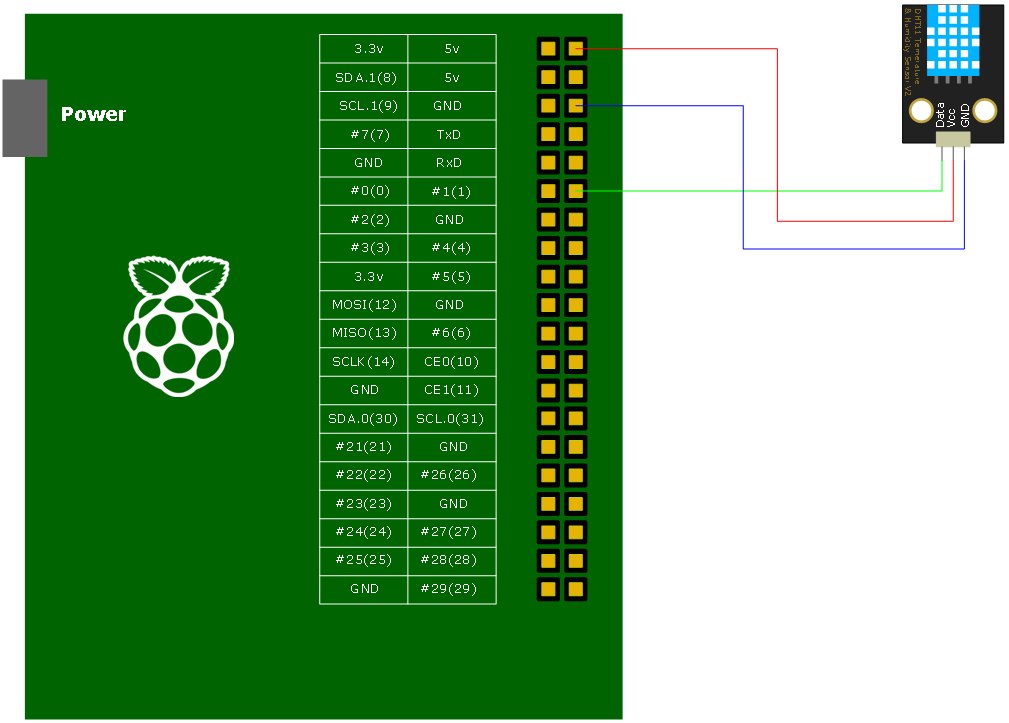
\includegraphics[width=200px]{./images/raspberry/dht11test.png}
\caption{DHT11 Sensor Test}
\label{fig:dht11_epics_test}
\end{figure}
최종 목표는 다음 Record를 만들어 온습도 값을 읽는 것이다.
\begin{lstlisting}[style=termstyle]
record(ai, "tem")
{
  field(DTYP, "DHT11")
  field(SCAN, "1 second")
  field(INP, "@1 temperature")
}

record(ai, "hum")
{
  field(DTYP, "DHT11")
  field(SCAN, "1 second")
  field(INP, "@1 humidity")
}
\end{lstlisting}
siteApps안에 dht11폴더를 만든 후 Base Application을 생성한다.
\begin{lstlisting}[style=termstyle]
pi@ctrlpi3 cd ../epics/R3.14.12.4/siteApps
pi@ctrlpi3 ~/epics/R3.14.12.4/siteApps $ mkdir dht11
pi@ctrlpi3 ~/epics/R3.14.12.4/siteApps $ cd dht11
pi@ctrlpi3 ~/epics/R3.14.12.4/siteApps/dht11 $ makeBaseApp.pl -t ioc dht11
pi@ctrlpi3 ~/epics/R3.14.12.4/siteApps/dht11 $ makeBaseApp.pl -i -t ioc dht11

Using target architecture linux-arm (only one available)
The following applications are available:
    dht11
What application should the IOC(s) boot?
The default uses the IOC's name, even if not listed above.
Application name?

pi@ctrlpi3 ~/epics/R3.14.12.4/siteApps/dht11 $ ls
conigure  dht11App  iocBoot Makefile
\begin{lstlisting}[style=termstylenumber, caption={Editing \texttt{/etc/fai/NFSROOT}}, label={list:nfsroot-file}]
#include <stdio.h>
#include <string.h>
#include <stdlib.h>

#include <epicsExport.h>
#include <devSup.h>
#include <recSup.h>
#include <recGbl.h>
#include <dbAccess.h>
#include <callback.h>
#include <aiRecord.h>

#include <wiringPi.h>

static long ai_init_record(aiRecord *pai);
static long read_ai(aiRecord *pai);

static long ai_init_record(aiRecord *pai)
{
}
	
static long read_ai(aiRecord *pai)
{
}

struct
{
  long num;
  DEVSUPFUN     report;
  DEVSUPFUN     init;
  DEVSUPFUN     init_record;
  DEVSUPFUN     get_ioint_info;
  DEVSUPFUN     read_ai;
  DEVSUPFUN     special_linconv;
} devAiDHT11Async = {
  6,
  NULL,
  NULL,
  ai_init_record,
  NULL,
  read_ai,
  NULL
};

epicsExportAddress(dset,devAiDHT11Async);
\end{lstlisting}
기본 구조는 아날로그 입력을 위해 aiRecord를 사용하였으며, 초기화 함수와 센서 값을 읽기 위한 함수로
구성되어 있다. 또한 wiringPi Library를 사용하기 위해 헤더파일을 추가하였다. dset을 devAiDHT11Async로 
설정하였으므로 devDHT11.dbd 파일을 만들어 다음과 같이 작성한다. 
\begin{lstlisting}[style=termstyle]
device(ai, INST_IO, devAiDHT11Async, "DHT11")
\end{lstlisting}
이제 실제 코드를 작성하도록 한다. 우선 코드를 Asynchronous 형식으로 만들기 위해 다음과 같이 Callback 
함수를 만들고 초기화 한다. 
\begin{lstlisting}[style=termstylenumber, caption={Editing \texttt{/etc/fai/NFSROOT}}, label={list:nfsroot-file}]
#include <stdio.h>
#include <string.h>
#include <stdlib.h>

#include <epicsExport.h>
#include <devSup.h>
#include <recSup.h>
#include <recGbl.h>
#include <dbAccess.h>
#include <callback.h>
#include <aiRecord.h>

#include <wiringPi.h>

typedef struct _DHT_INFO
{
  CALLBACK callback;

}DHT_INFO;

static long ai_init_record(aiRecord *pai);
static long read_ai(aiRecord *pai);

static void myCallback(CALLBACK *pcallback)
{
  aiRecord *precord;
  struct rset *prset;

  callbackGetUser(precord, pcallback);
  prset = (struct rset *)(precord->rset);

  dbScanLock((dbCommon*)precord);
  (*prset->process)(precord);
  dbScanUnlock((dbCommon*)precord);
}

static long ai_init_record(aiRecord *pai)
{
  DHT_INFO *dht_info = malloc(sizeof(DHT_INFO));

  callbackSetCallback(myCallback, &dht_info->callback);
  callbackSetPriority(priorityLow, &dht_info->callback);
  callbackSetUser(pai, &dht_info->callback);

  pai->dpvt = dht_info;
}
	
static long read_ai(aiRecord *pai)
{
  DHT_INFO *dht_info = pai->dpvt;

  if(pai->pact)
  {
    pai->udf = FALSE;

    return 2;
  }

  pai->pact = TRUE;
  callbackRequestDelayed(&dht_info->callback, pai->disv);

  return 0;

}

struct
{
  long num;
  DEVSUPFUN     report;
  DEVSUPFUN     init;
  DEVSUPFUN     init_record;
  DEVSUPFUN     get_ioint_info;
  DEVSUPFUN     read_ai;
  DEVSUPFUN     special_linconv;
} devAiDHT11Async = {
  6,
  NULL,
  NULL,
  ai_init_record,
  NULL,
  read_ai,
  NULL
};

epicsExportAddress(dset,devAiDHT11Async);
\end{lstlisting}
DHT\_INFO 구조체는 callback 함수의 포인터를 포함하여 센서에 대한 정보를 저장하기 위한 구조체 이다.
기본적인 준비가 되었으므로 몇가지 초기화 작업을 다음과 같이 추가한다.
\begin{lstlisting}[style=termstylenumber, caption={Editing \texttt{/etc/fai/NFSROOT}}, label={list:nfsroot-file}]
static long ai_init_record(aiRecord *pai)
{
  DHT_INFO *dht_info = malloc(sizeof(DHT_INFO));

  callbackSetCallback(myCallback, &dht_info->callback);
  callbackSetPriority(priorityLow, &dht_info->callback);
  callbackSetUser(pai, &dht_info->callback);

  if(wiringPiSetup() == -1)
    return 1;

  char *para;
  char *sensor;
  int pin_num = 0;
  int mode = 0;

  para = pai->inp.value.instio.string;

  pin_num = atoi(strtok(para, " "));
  sensor = strtok(NULL, " ");

  if(strcmp(sensor, "humidity") == 0)
    mode = 0;
  else
    mode = 1;

  pai->dpvt = dht_info;
  
  return 0;
}
\end{lstlisting}
다음에는 Record에서 설정한 Pin번호와 Read Type(Humidity 또는 Temperature)를 읽어 공백을 기준으로 분리해서
각각 변수에 저장한다. 참고로 atoi는 문자열을 정수형으로 변환해주는 C Library 함수이고, strtok는 문자열을
분리 문자를 기준으로 문자를 분리해서 반환시켜 준다.
\begin{lstlisting}[style=termstyle]
para = pai->inp.value.instio.string;

pin_num = atoi(strtok(para, " "));
sensor = strtok(NULL, " ");
\end{lstlisting}
이제 분리된 문자중 Read Type에 따라 mode 값을 설정한다.
\begin{lstlisting}[style=termstyle]
if(strcmp(sensor, "humidity") == 0)
  mode = 0;
else
  mode = 1;
\end{lstlisting}
지금까지 저장된 pin\_num과 mode값을 read\_ai 함수에서 사용하기 위해 다음과 같이 DHT\_INFO 구조체에 
변수를 추가하고 값을 Pin Number와 Mode로 초기화 한다.
\begin{lstlisting}[style=termstylenumber, caption={Editing \texttt{/etc/fai/NFSROOT}}, label={list:nfsroot-file}]
struct _DHT_INFO
{	
  CALLBACK callback;

  int pin_num;
  int pin_mode;

}DHT_INFO;

...
...

static long ai_init_record(aiRecord *pai)
{
  DHT_INFO *dht_info = malloc(sizeof(DHT_INFO));

  callbackSetCallback(myCallback, &dht_info->callback);
  callbackSetPriority(priorityLow, &dht_info->callback);
  callbackSetUser(pai, &dht_info->callback);

  if(wiringPiSetup() == -1)
    return 1;

  char *para;
  char *sensor;
  int pin_num = 0;
  int mode = 0;

  para = pai->inp.value.instio.string;

  pin_num = atoi(strtok(para, " "));
  sensor = strtok(NULL, " ");

  if(strcmp(sensor, "humidity") == 0)
    mode = 0;
  else
    mode = 1;

  dht_info->pin_num = pin_num;
  dht_info->pin_mode = mode;

  pai->dpvt = dht_info;

  return 0;
}
\end{lstlisting}
다음은 read\_ai 함수에 실제 값을 읽어 Record 변수에 저장하는 코드를 추가한다.
\begin{lstlisting}[style=termstylenumber, caption={Editing \texttt{/etc/fai/NFSROOT}}, label={list:nfsroot-file}]
static long read_ai(aiRecord *pai)
{
  DHT_INFO *dht_info = pai->dpvt;

  if(pai->pact)
  {
    readDHT11(dht_info);

    if(dht_info->pin_mode == 0)
      pai->val = dht_info->val_h;
    else
      pai->val = dht_info->val_t;

    pai->udf = FALSE;

    return 2;
  }

  pai->pact = TRUE;
  callbackRequestDelayed(&dht_info->callback, pai->disv);

  return 0;
}
\end{lstlisting}
readDHT11 함수는 실제 센서로 부터 온습도 값을 읽은 후 DHT\_INFO 구조체에 선언된 온습도 변수에 저장하는 
함수로 다음과 같다.
\begin{lstlisting}[style=termstylenumber, caption={Editing \texttt{/etc/fai/NFSROOT}}, label={list:nfsroot-file}]
void readDHT11(DHT_INFO *dht_info)
{
  int pin = dht_info->pin_num;
  int mode = dht_info->pin_mode;
  
  int i=0;
  for(i=0;i<5;i++)
      dht11_val[i]=0;

  epicsUInt8 lststate=HIGH;
  epicsUInt8 counter=0;
  epicsUInt8 j=0,i;

  pinMode(pin,OUTPUT);
  digitalWrite(pin,LOW);
  delay(18);
  digitalWrite(pin,HIGH);
  delayMicroseconds(40);
  pinMode(pin,INPUT);

  int j=0;
  for(i=0;i<MAX_TIME;i++)
  {
    counter=0;
    while(digitalRead(pin)==lststate)
    {
      counter++;
      delayMicroseconds(1);
      if(counter==255)
	break;
    }

    lststate=digitalRead(pin);
    if(counter==255)
       break;
    // top 3 transistions are ignored
    if((i>=4)&&(i%2==0))
    {
      dht11_val[j/8]<<=1;
      if(counter>16)
	dht11_val[j/8]|=1;
      j++;
    }
  }

  float val = 0.0f;
  char tmp[10];

  sprintf(tmp, "%d.%d", dht11_val[0], dht11_val[1]);
  val = atof(tmp);

  dht_info->val_h = val;

  sprintf(tmp, "%d.%d", dht11_val[2], dht11_val[3]);
  val = atof(tmp);

  dht_info->val_t = val;
}
\end{lstlisting}
dht11\_val배열, 함수이름, MAX\_TIME를 헤더 선언 아래에 추가해 주고 온습도 값을 저장하는 변수를 
DHT\_INFO구조체 안에 선언해 준다. 초기화 함수에는 dht11\_val 배열과 구조체 변수를 0으로 초기화 하는 
코드를 추가한다.
\begin{lstlisting}[style=termstylenumber, caption={Editing \texttt{/etc/fai/NFSROOT}}, label={list:nfsroot-file}]
#include <wiringPi.h>

#define MAX_TIME 85

int dht11_val[5];

typedef struct _DHT_INFO
{
  CALLBACK callback;

  int pin_num;
  int pin_mode;

  float val_h;
  float val_t;

}DHT_INFO;

void readDHT11(DHT_INFO *dht_info);

static long ai_init_record(aiRecord *pai);
static long read_ai(aiRecord *pai);

static long ai_init_record(aiRecord *pai)
{
  ...
  ...

  if(strcmp(sensor, "humidity") == 0)
    mode = 0;
  else
    mode = 1;

  int i;
  for(i=0;i<5;i++)
  {
    dht11_val[i] = 0;
  }

  dht_info->val_h = 0.0f;
  dht_info->val_t = 0.0f;

...
...
}
\end{lstlisting}
지금까지 작성한 readDHT11 함수는 유효성 검사가 빠져있다. 따라서 잘못된 온습도 센서 값이 읽어지면 그대로
출력하는 문제점이 있다. 이러한 문제를 해결하기 위해 유효성 검사코드를 추가한다. 유효성 검사는 dth22\_val 
배열의 마지막 checksum 값이 나머지 4개의 값의 합과 같은 경우에만 올바른 값으로 볼 수 있다. 만약 checksum
값과 차이가 발생 할 경우 이전 값을 유지하도록 한다. 참고로 checksum을 검사하는 방법은 센서 또는 장비마다 
다르므로 메뉴얼을 참고한다.
\begin{lstlisting}[style=termstylenumber, caption={Editing \texttt{/etc/fai/NFSROOT}}, label={list:nfsroot-file}]
void readDHT11(DHT_INFO *dht_info)
{
  int pin = dht_info->pin_num;
  int mode = dht_info->pin_mode;
  
  int i=0;
  for(i=0;i<5;i++)
      dht11_val[i]=0;

  epicsUInt8 lststate=HIGH;
  epicsUInt8 counter=0;
  epicsUInt8 j=0,i;

  pinMode(pin,OUTPUT);
  digitalWrite(pin,LOW);
  delay(18);
  digitalWrite(pin,HIGH);
  delayMicroseconds(40);
  pinMode(pin,INPUT);

  int j=0;
  for(i=0;i<MAX_TIME;i++)
  {
    counter=0;
    while(digitalRead(pin)==lststate)
    {
      counter++;
      delayMicroseconds(1);
      if(counter==255)
	break;
    }

    lststate=digitalRead(pin);
    if(counter==255)
       break;
    // top 3 transistions are ignored
    if((i>=4)&&(i%2==0))
    {
      dht11_val[j/8]<<=1;
      if(counter>16)
	dht11_val[j/8]|=1;
      j++;
    }
  }

  float val = 0.0f;
  char tmp[10];
  if((j>=40)&&(dht11_val[4]==((dht11_val[0]+dht11_val[1]+dht11_val[2]+dht11_val[3])& 0xFF)))
  {
    sprintf(tmp, "%d.%d", dht11_val[0], dht11_val[1]);
    val = atof(tmp);

    dht_info->val_h = val;
    dht_info->pre_val_h = h;

    sprintf(tmp, "%d.%d", dht11_val[2], dht11_val[3]);
    val = atof(tmp);

    dht_info->val_t = val;
    dht_info->pre_val_t = t;
  }
  else
  {
    if(mode == 0)
      dht_info->val_h = dht_info->pre_val_h;
    else
      dht_info->val_t = dht_info->pre_val_t;
  }

}
\end{lstlisting}
pre\_val\_h와 pre\_val\_t 변수는 이전 온습도 값을 가지고 있어 유효성 검사가 실패할 경우 이전 값을 다시 
돌려준다. 두 변수를 DHT\_INFO 구조체 안에 선언해 주고 초기화 코드를 넣는다. 
\begin{lstlisting}[style=termstylenumber, caption={Editing \texttt{/etc/fai/NFSROOT}}, label={list:nfsroot-file}]
#include <wiringPi.h>
#define MAX_TIME 85

int dht11_val[5];

typedef struct _DHT_INFO
{
  CALLBACK callback;

  int pin_num;
  int pin_mode;

  float val_h;
  float val_t;

  float pre_val_h;
  float pre_val_t;

}DHT_INFO;

...
...

static long ai_init_record(aiRecord *pai)
{
  ...
  ...

  if(strcmp(sensor, "humidity") == 0)
    mode = 0;
  else
    mode = 1;

  int i;
  for(i=0;i<5;i++)
  {
    dht11_val[i] = 0;
  }
  
  dht_info->val_h = 0.0f;
  dht_info->val_t = 0.0f;
  dht_info->pre_val_h = 0.0f;
  dht_info->pre_val_t = 0.0f;

  ...
  ...

}
\end{lstlisting}
전체 코드는 아래와 같다.
\begin{lstlisting}[style=termstylenumber, caption={Editing \texttt{/etc/fai/NFSROOT}}, label={list:nfsroot-file}]
#include <stdio.h>
#include <string.h>
#include <stdlib.h>

#include <epicsExport.h>
#include <devSup.h>
#include <recSup.h>
#include <recGbl.h>
#include <dbAccess.h>
#include <callback.h>
#include <aiRecord.h>

#include <wiringPi.h>

#define MAX_TIME 85

int dht11_val[5];

typedef struct _DHT_INFO
{
  CALLBACK callback;

  int pin_num;
  int pin_mode;

  float val_h;
  float val_t;

  float pre_val_h;
  float pre_val_t;
}DHT_INFO;

void readDHT11(DHT_INFO *dht_info);

static long ai_init_record(aiRecord *pai);
static long read_ai(aiRecord *pai);

static void myCallback(CALLBACK *pcallback)
{
  aiRecord *precord;
  struct rset *prset;

  callbackGetUser(precord, pcallback);
  prset = (struct rset *)(precord->rset);

  dbScanLock((dbCommon*)precord);
  (*prset->process)(precord);
  dbScanUnlock((dbCommon*)precord);
}

static long ai_init_record(aiRecord *pai)
{
  DHT_INFO *dht_info = malloc(sizeof(DHT_INFO));

  callbackSetCallback(myCallback, &dht_info->callback);
  callbackSetPriority(priorityLow, &dht_info->callback);
  callbackSetUser(pai, &dht_info->callback);

  if(wiringPiSetup() == -1)
    return 1;

  char *para;
  char *sensor;
  int pin_num = 0;
  int mode = 0;

  para = pai->inp.value.instio.string;

  pin_num = atoi(strtok(para, " "));
  sensor = strtok(NULL, " ");

  if(strcmp(sensor, "humidity") == 0)
    mode = 0;
  else
    mode = 1;

  int i;
  for(i=0;i<5;i++)
    dht11_val[i] = 0;

  dht_info->val_h = 0.0f;
  dht_info->val_t = 0.0f;
  dht_info->pre_val_h = 0.0f;
  dht_info->pre_val_t = 0.0f;

  dht_info->pin_num = pin_num;
  dht_info->pin_mode = mode;

  pai->dpvt = dht_info;

  return 0;
}

static long read_ai(aiRecord *pai)
{
  DHT_INFO *dht_info = pai->dpvt;

  if(pai->pact)
  {
    readDHT11(dht_info);

    if(dht_info->pin_mode == 0)
      pai->val = dht_info->val_h;
    else
      pai->val = dht_info->val_t;

    pai->udf = FALSE;

    return 2;
  }

  pai->pact = TRUE;
  callbackRequestDelayed(&dht_info->callback, pai->disv);

  return 0;
}

struct
{
  long num;
  DEVSUPFUN     report;
  DEVSUPFUN     init;
  DEVSUPFUN     init_record;
  DEVSUPFUN     get_ioint_info;
  DEVSUPFUN     read_ai;
  DEVSUPFUN     special_linconv;
} devAiDHT11Async = {
  6,
  NULL,
  NULL,
  ai_init_record,
  NULL,
  read_ai,
  NULL
};

epicsExportAddress(dset,devAiDHT11Async);

void readDHT11(DHT_INFO *dht_info)
{
  int pin = dht_info->pin_num;
  int mode = dht_info->pin_mode;

  int i=0;
  for(i=0;i<5;i++)
      dht11_val[i]=0;

  epicsUInt8 lststate=HIGH;
  epicsUInt8 counter=0;

  pinMode(pin,OUTPUT);
  digitalWrite(pin,LOW);
  delay(18);
  digitalWrite(pin,HIGH);
  delayMicroseconds(40);
  pinMode(pin,INPUT);

  int j=0;
  for(i=0;i<MAX_TIME;i++)
  {
    counter=0;
    while(digitalRead(pin)==lststate)
    {
      counter++;
      delayMicroseconds(1);
      if(counter==255)
	break;
    }

    lststate=digitalRead(pin);
    if(counter==255)
       break;
    // top 3 transistions are ignored
    if((i>=4)&&(i%2==0))
    {
      dht11_val[j/8]<<=1;
      if(counter>16)
	dht11_val[j/8]|=1;
      j++;
    }
  }

  float val = 0.0f;
  char tmp[10];

  if((j>=40)&&(dht11_val[4]==((dht11_val[0]+dht11_val[1]+dht11_val[2]+dht11_val[3])& 0xFF)))
  {
    sprintf(tmp, "%d.%d", dht11_val[0], dht11_val[1]);
    val = atof(tmp);

    dht_info->val_h = val;
    dht_info->pre_val_h = val;

    sprintf(tmp, "%d.%d", dht11_val[2], dht11_val[3]);
    val = atof(tmp);

    dht_info->val_t = val;
    dht_info->pre_val_t = val;
  }
  else
  {
    if(mode == 0)
      dht_info->val_h = dht_info->pre_val_h;
    else
      dht_info->val_t = dht_info->pre_val_t;
  }
}
\end{lstlisting}
마지막으로 Makefile에 다음 코드를 추가한 후 make를 실행한다.
\begin{lstlisting}[style=termstyle]
TOP=../..

include $(TOP)/configure/CONFIG
#----------------------------------------
#  ADD MACRO DEFINITIONS AFTER THIS LINE
#=============================

#=============================
# Build the IOC application

USR_INCLUDES += -I/home/pi/wiringPi/wiringPi
wiringPi_DIR += /home/pi/wiringPi/wiringPi /home/pi/wiringPi/devLib

PROD_IOC = dht11
# dht11.dbd will be created and installed
DBD += dht11.dbd

# dht11.dbd will be made up from these files:
dht11_DBD += base.dbd

# Include dbd files from all support applications:
#dht11_DBD += xxx.dbd
dht11_DBD += devDHT11.dbd

# Add all the support libraries needed by this IOC
#dht11_LIBS += xxx

# dht11_registerRecordDeviceDriver.cpp derives from dht11.dbd
dht11_SRCS += dht11_registerRecordDeviceDriver.cpp
dht11_SRCS += devDHT11.c

# Build the main IOC entry point on workstation OSs.
dht11_SRCS_DEFAULT += dht11Main.cpp
dht11_SRCS_vxWorks += -nil-

# Add support from base/src/vxWorks if needed
#dht11_OBJS_vxWorks += $(EPICS_BASE_BIN)/vxComLibrary

# Finally link to the EPICS Base libraries
dht11_LIBS += $(EPICS_BASE_IOC_LIBS)
dht11_LIBS += wiringPi

#===========================

include $(TOP)/configure/RULES
#----------------------------------------
#  ADD RULES AFTER THIS LINE
\end{lstlisting}
\begin{lstlisting}[style=termstyle]
pi@ctrlpi3 ~/epics/R3.14.12.4/siteApps/dht11/dht11App/src $ make
\end{lstlisting}
make가 완료되면 bin/linux-arm 폴더에 dht11 파일이 생성된다.
테스트를 위해 dht11App/Db 폴더로 이동한 후 처음 테스트 하고자 했던 dht11.db 파일을 만든다.
\begin{lstlisting}[style=termstyle]
record(ai, "tem")
{
  field(DTYP, "DHT11")
  field(SCAN, "1 second")
  field(INP, "@1 temperature")
}

record(ai, "hum")
{
  field(DTYP, "DHT11")
  field(SCAN, "1 second")
  field(INP, "@1 humidity")
}
\end{lstlisting}
Makefile에 dth11.db를 추가한 후 make를 실행한다.
\begin{lstlisting}[style=termstyle]
TOP=../..
include $(TOP)/configure/CONFIG
#----------------------------------------
#  ADD MACRO DEFINITIONS AFTER THIS LINE

#----------------------------------------------------
#  Optimization of db files using dbst (DEFAULT: NO)
#DB_OPT = YES

#----------------------------------------------------
# Create and install (or just install) into /db
# databases, templates, substitutions like this
#DB += xxx.db
DB += dht11.db

#----------------------------------------------------
# If .db template is not named *.template add
# _template = 

include $(TOP)/configure/RULES
#----------------------------------------
#  ADD RULES AFTER THIS LINE
\end{lstlisting}
\begin{lstlisting}[style=termstyle]
pi@ctrlpi3 ~/epics/R3.14.12.4/siteApps/dht11/dht11App/Db $ make
\end{lstlisting}
make가 완료되면 최상위 폴더에 db폴더가 만들어지고 그 안에 dht11.db파일이 생성된다.
\begin{lstlisting}[style=termstyle]
pi@ctrlpi3 ~/epics/R3.14.12.4/siteApps/dht11/db $ ls
dht11.db
\end{lstlisting}
이제 ioc를 실행하기 위해 iocBoot/iocdht11 폴더로 이동한다.
st.cmd파일을 수정하기 전 make를 실행해서 envPahts파일을 만든다.
\begin{lstlisting}[style=termstyle]
pi@ctrlpi3 ~/epics/R3.14.12.4/siteApps/dht11/iocBoot/iocdht11 $ make
pi@ctrlpi3 ~/epics/R3.14.12.4/siteApps/dht11/iocBoot/iocdht11 $ ls
envPaths  Makefile  st.cmd
\end{lstlisting}
이제 st.cmd파일을 열어 dht11.db 레코드를 추가해 준다.
\begin{lstlisting}[style=termstyle]
#!../../bin/linux-arm/dht11

## You may have to change dht11 to something else
## everywhere it appears in this file

< envPaths

cd ${TOP}

## Register all support components
dbLoadDatabase "dbd/dht11.dbd"
dht11_registerRecordDeviceDriver pdbbase

## Load record instances
#dbLoadRecords("db/xxx.db","user=piHost")
dbLoadRecords("db/dht11.db")

cd ${TOP}/iocBoot/${IOC}
iocInit

## Start any sequence programs
#seq sncxxx,"user=piHost"
\end{lstlisting}
최종적으로 st.cmd 파일을 실행파일로 변경한 후 실행한다.
\begin{lstlisting}[style=termstyle]
pi@ctrlpi3 ~/epics/R3.14.12.4/siteApps/dht11/iocBoot/iocdht11 $ chmod 755 st.cmd
pi@ctrlpi3 ~/epics/R3.14.12.4/siteApps/dht11/iocBoot/iocdht11 $ sudo ./st.cmd
#!../../bin/linux-arm/dht11
## You may have to change dht11 to something else
## everywhere it appears in this file
< envPaths
epicsEnvSet("ARCH","linux-arm")
epicsEnvSet("IOC","iocdht11")
epicsEnvSet("TOP","/home/pi/epics/R3.14.12.4/siteApps/dht11")
epicsEnvSet("EPICS_BASE","/home/pi/epics/R3.14.12.4/base")
cd /home/pi/epics/R3.14.12.4/siteApps/dht11
## Register all support components
dbLoadDatabase "dbd/dht11.dbd"
dht11_registerRecordDeviceDriver pdbbase
## Load record instances
#dbLoadRecords("db/xxx.db","user=piHost")
dbLoadRecords("db/dht11.db")
cd /home/pi/epics/R3.14.12.4/siteApps/dht11/iocBoot/iocdht11
iocInit
Starting iocInit
############################################################################
## EPICS R3.14.12.4 $Date: Mon 2013-12-16 15:51:45 -0600$
## EPICS Base built Aug 29 2014
############################################################################
iocRun: All initialization complete
## Start any sequence programs
#seq sncxxx,"user=piHost"
epics> 
\end{lstlisting}
온도와 습도값이 제대로 읽어지면 끝!
\begin{lstlisting}[style=termstyle]
epics> dbpr tem
ASG:                DESC:               DISA: 0             DISP: 0             
DISV: 1             NAME: tem           RVAL: 0             SEVR: NO_ALARM      
STAT: NO_ALARM      SVAL: 0             TPRO: 0             VAL: 26     
epics> dbpr hum
ASG:                DESC:               DISA: 0             DISP: 0             
DISV: 1             NAME: hum           RVAL: 57            SEVR: NO_ALARM      
STAT: NO_ALARM      SVAL: 0             TPRO: 0             VAL: 57 
\end{lstlisting}

\subsection{DHT22}
\subsection{DS1820}
본 메뉴얼에서는 다음과 같은 하드웨어 구성과 EPICS Record를 만들어 DS1820센서의 온도 값을 읽는 Library를 만드는 것이다. 여기서 "@1"은 GPIO Pin 번호를 의미한다.

하드웨어 구성은 다음과 같다.
\begin{itemize}
\item Raspberry Pi Model B+
\item DS1820 Sensor
\item 4.7k Ohme Register
\end{itemize}
\begin{figure}[!htb]
\centering
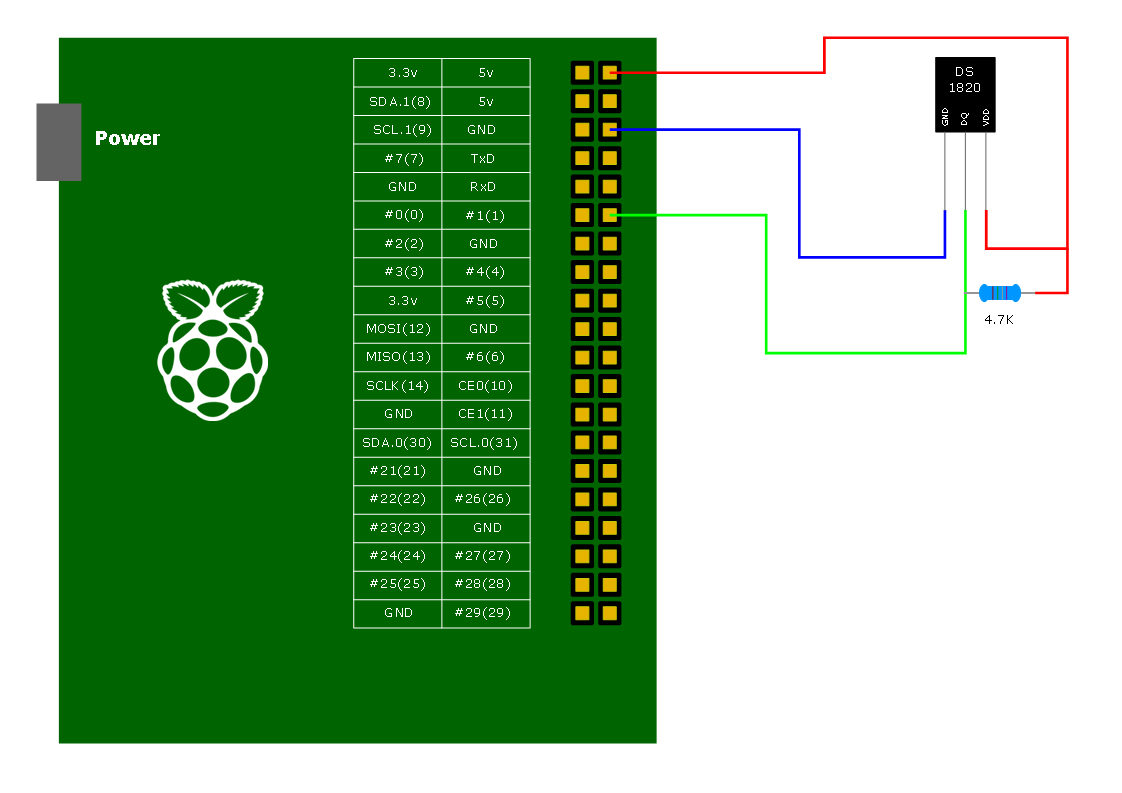
\includegraphics[width=1\textwidth]{./images/raspberry/ds1820_test.png}
\caption{DS1820 Sensor Test}
\label{fig:ds1820_epics_test}
\end{figure}
최종 목표는 다음 Record를 만들어 온습도 값을 읽는 것이다.
\begin{lstlisting}[style=termstyle]
record(ai, "ds1820")       
{
 field(DTYP, "DS1820")
  field(SCAN, "1 second")
  field(INP, "@1")
}
\end{lstlisting}
siteApps안에 ds1820폴더를 만든 후 Base Application을 생성한다.
\begin{lstlisting}[style=termstyle]
pi@raspberrypi cd ../epics/R3.14.12.4/siteApps
pi@raspberrypi ~/epics/R3.14.12.4/siteApps $ mkdir ds1820
pi@raspberrypi ~/epics/R3.14.12.4/siteApps $ cd ds1820
pi@raspberrypi ~/epics/R3.14.12.4/siteApps/ds1820 $ makeBaseApp.pl -t ioc ds1820
pi@raspberrypi ~/epics/R3.14.12.4/siteApps/ds1820 $ makeBaseApp.pl -i -t ioc ds1820

Using target architecture linux-arm (only one available)
The following applications are available:
    ds1820
What application should the IOC(s) boot?
The default uses the IOC's name, even if not listed above.
Application name?

pi@raspberrypi ~/epics/R3.14.12.4/siteApps/ds1820 $ ls
conigure  ds1820App  iocBoot Makefile
\end{lstlisting}
ds1820App/src 폴더로 이동한 후 devDS1820.c 파일을 만들어 기본 코드를 작성한다.
\begin{lstlisting}[style=termstylenumber, caption={Editing \texttt{/etc/fai/NFSROOT}}, label={list:nfsroot-file}]
#include <stdio.h>
#include <string.h>
#include <stdlib.h>

#include <epicsExport.h>
#include <devSup.h>
#include <recSup.h>
#include <recGbl.h>
#include <dbAccess.h>
#include <callback.h>
#include <aiRecord.h>

#include <wiringPi.h>

static long ai_init_record(aiRecord *pai);
static long read_ai(aiRecord *pai);

static long ai_init_record(aiRecord *pai)
{
}

static long read_ai(aiRecord *pai)
{
}

struct
{
  long num;
  DEVSUPFUN     report;
  DEVSUPFUN     init;
  DEVSUPFUN     init_record;
  DEVSUPFUN     get_ioint_info;
  DEVSUPFUN     read_ai;
  DEVSUPFUN     special_linconv;
} devAiDS1820Async = {
  6,
  NULL,
  NULL,
  ai_init_record,
  NULL,
  read_ai,
  NULL
};

epicsExportAddress(dset,devAiDS1820Async);
\end{lstlisting}
기본 구조는 아날로그 입력을 위해 aiRecord를 사용하였으며, 초기화 함수와 센서 값을 읽기 위한 함수로 
구성되어 있다. 또한 wiringPi Library를 사용하기 위해 헤더파일을 추가하였다. dset을 devAiDS1820Async로 
설정하였으므로 devDS1820.dbd 파일을 만들어 다음과 같이 작성한다.
\begin{lstlisting}[style=termstyle]
device(ai, INST_IO, devAiDS1820Async, "DS1820")
\end{lstlisting}
이제 실제 코드를 작성하도록 한다. 우선 코드를 Asynchronous 형식으로 만들기 위해 다음과 같이 Callback 
함수를 만들고 초기화 한다. 
\begin{lstlisting}[style=termstylenumber, caption={Editing \texttt{/etc/fai/NFSROOT}}, label={list:nfsroot-file}]
#include <stdio.h>
#include <string.h>
#include <stdlib.h>

#include <epicsExport.h>
#include <devSup.h>
#include <recSup.h>
#include <recGbl.h>
#include <dbAccess.h>
#include <callback.h>
#include <aiRecord.h>

#include <wiringPi.h>

typedef struct _DS1820_INFO
{
  CALLBACK callback;

}DS1820_INFO;

static long ai_init_record(aiRecord *pai);
static long read_ai(aiRecord *pai);

static void myCallback(CALLBACK *pcallback)
{
  aiRecord *precord;
  struct rset *prset;

  callbackGetUser(precord, pcallback);
  prset = (struct rset *)(precord->rset);

  dbScanLock((dbCommon*)precord);
  (*prset->process)(precord);
  dbScanUnlock((dbCommon*)precord);
}

static long ai_init_record(aiRecord *pai)
{
  DS1820_INFO *ds1820_info = malloc(sizeof(DS1820_INFO));

  callbackSetCallback(myCallback, &ds1820_info->callback);
  callbackSetPriority(priorityLow, &ds1820_info->callback);
  callbackSetUser(pai, &ds1820_info->callback);

  pai->dpvt = ds1820_info;
}

static long read_ai(aiRecord *pai)
{
  DS1820_INFO *ds1820_info = pai->dpvt;

  if(pai->pact)
  {
    pai->udf = FALSE;

    return 2;
  }

  pai->pact = TRUE;
  callbackRequestDelayed(&ds1820_info->callback, pai->disv);

  return 0;

}

struct
{
  long num;
  DEVSUPFUN     report;
  DEVSUPFUN     init;
  DEVSUPFUN     init_record;
  DEVSUPFUN     get_ioint_info;
  DEVSUPFUN     read_ai;
  DEVSUPFUN     special_linconv;
} devAiDS1820Async = {
  6,
  NULL,
  NULL,
  ai_init_record,
  NULL,
  read_ai,
  NULL
};

epicsExportAddress(dset,devAiDS1820Async);
\end{lstlisting}
DS1820\_INFO 구조체는 callback 함수의 포인터를 포함하여 센서에 대한 정보를 저장하기 위한 구조체 이다.
기본적인 준비가 되었으므로 몇가지 초기화 작업을 다음과 같이 추가한다.
\begin{lstlisting}[style=termstylenumber, caption={Editing \texttt{/etc/fai/NFSROOT}}, label={list:nfsroot-file}]
static long ai_init_record(aiRecord *pai)
{
  DS1820_INFO *ds1820_info = malloc(sizeof(DS1820_INFO));

  callbackSetCallback(myCallback, &ds1820_info->callback);
  callbackSetPriority(priorityLow, &ds1820_info->callback);
  callbackSetUser(pai, &ds1820_info->callback);

  if(wiringPiSetup() == -1)
    return 1;

  char *para;
  int pin_num = 0;

  para = pai->inp.value.instio.string;

  pin_num = atoi(para);

  pai->dpvt = ds1820_info;

  return 0;
}
\end{lstlisting}
pin\_num를 read\_ai 함수에서 사용하기 위해 다음과 같이 DS1820\_INFO 구조체에 변수를 추가하고 값을 초기화 
한다.
\begin{lstlisting}[style=termstylenumber, caption={Editing \texttt{/etc/fai/NFSROOT}}, label={list:nfsroot-file}]
struct _DS1820_INFO
{
  CALLBACK callback;

  int pin_num;

}DS1820_INFO;

...
...

static long ai_init_record(aiRecord *pai)
{
  DS1820_INFO *ds1820_info = malloc(sizeof(DS1820_INFO));

  callbackSetCallback(myCallback, &ds1820_info->callback);
  callbackSetPriority(priorityLow, &ds1820_info->callback);
  callbackSetUser(pai, &ds1820_info->callback);

  if(wiringPiSetup() == -1)
    return 1;

  char *para;
  int pin_num = 0;

  para = pai->inp.value.instio.string;

  pin_num = atoi(para);


  ds1820_info->pin_num = pin_num;

  pai->dpvt = ds1820_info;

  return 0;
}
\end{lstlisting}
다음은 read\_ai 함수에 실제 값을 읽어 Record 변수에 저장하는 코드를 추가한다.
\begin{lstlisting}[style=termstylenumber, caption={Editing \texttt{/etc/fai/NFSROOT}}, label={list:nfsroot-file}]
static long read_ai(aiRecord *pai)
{
  DS1820_INFO *ds1820_info = pai->dpvt;

  if(pai->pact)
  {
  readDS1820(ds1820_info);

    pai->val = ds1820_info->temper;

    pai->udf = FALSE;

    return 2;
  }

  pai->pact = TRUE;
  callbackRequestDelayed(&dht_info->callback, pai->disv);

  return 0;
}
\end{lstlisting}
readDS1820 함수는 실제 센서로 부터 온습도 값을 읽은 후 DS1820\_INFO 구조체에 선언된 온습도 변수에 저장하는 
함수로 다음과 같다. 
\begin{lstlisting}[style=termstylenumber, caption={Editing \texttt{/etc/fai/NFSROOT}}, label={list:nfsroot-file}]
void ds1820_read(DS1820_INFO* ds1820_info)
{
  uint8_t busy = 1;
  int pin = ds1820_info->pin_num;

  onewire_reset(pin);
  onewire_write(pin, 0xCC);
  onewire_write(pin, 0x44);

  delay(750);
  while(busy == 0)
  {
    busy = onewire_read(pin);
    printf("busy: %d\n", busy);
  }

  onewire_reset(pin);
  onewire_write(pin, 0xCC);
  onewire_write(pin, 0xBE);

  uint8_t lsb, msb, th, tl, reserved1, reserved2, count_remain, count_per_c, crc;
  float real_temp = 0.0f;
  float pre_real_temp = ds1820_info->temper;
  signed char temp_read = 0;

  lsb = onewire_read(pin);
  msb = onewire_read(pin);
  th = onewire_read(pin);
  tl = onewire_read(pin);
  reserved1 = onewire_read(pin);
  reserved2 = onewire_read(pin);
  count_remain = onewire_read(pin);
  count_per_c = onewire_read(pin);
  crc = onewire_read(pin);

  uint8_t data[] = {lsb, msb, th, tl, reserved1, reserved2, count_remain, count_per_c};

  onewire_reset(pin);

  if(crc_read(data) == crc)
  {
    temp_read = (signed char)(lsb>>1);

    if(msb == 255)
      temp_read = temp_read | 0x80;

    real_temp = (float)temp_read + 0.85f - (float)count_remain/(float)count_per_c;
    real_temp = (int)(real_temp * 10) / 10.0f;

    ds1820_info->temper = real_temp;
    ds1820_info->pre_temper = real_temp;
  }
  else
    ds1820_info->temper = pre_real_temp;

}
\end{lstlisting}
ds1820\_read는 4개의 함수를 내부에서 호출하는데 다음과 같다.
\begin{itemize}
\item onewire\_reset: DS1820 센서를 초기화 한다.
\item onewire\_write: 8bit 정보를 센서로 전송한다.
\item onewire\_read: 8bit 정보를 센서로 부터 읽는다.
\item crc\_read: Cyclical Redundancy Check(CRC) 값을 계산한다.
\end{itemize}
onewire\_reset 함수는 DS1820 센서를 초기화 하는 함수로 다음과 같다.
\begin{lstlisting}[style=termstylenumber, caption={Editing \texttt{/etc/fai/NFSROOT}}, label={list:nfsroot-file}]
int onewire_reset(int pin)
{
  int result;

  pinMode(pin, OUTPUT);

  digitalWrite(pin, LOW);
  delayMicroseconds(480);

  pinMode(pin, INPUT);
  delayMicroseconds(70);

  result = digitalRead(pin);

  delayMicroseconds(410);

  return result;
}
\end{lstlisting}
 onewire\_write 함수는 8bit 정보를 센서로 전송하는 함수로 일정한 Timing에 맞춰 1bit씩 전송 하기위해 
onewire\_write\_bit 함수를 호출한다. 
\begin{lstlisting}[style=termstylenumber, caption={Editing \texttt{/etc/fai/NFSROOT}}, label={list:nfsroot-file}]
void onewire_write(int pin, uint8_t data)
{
  int loop;

  for(loop=0; loop<8; loop++)
  {
    onewire_write_bit(pin, data & 0x01);

    data >>= 1;
  }
}

void onewire_write_bit(int pin, int bit)
{
  pinMode(pin, OUTPUT);

  if(bit)
  {
    digitalWrite(pin, LOW);
    delayMicroseconds(6);
    digitalWrite(pin, HIGH);
    delayMicroseconds(64);
  }
  else
  {
    digitalWrite(pin, LOW);
    delayMicroseconds(60);
    digitalWrite(pin, HIGH);
    delayMicroseconds(10);
  }

}
\end{lstlisting}
 onewire\_read 함수는 onewire\_write 함수와 반대로 onewire\_read\_bit 함수를 통해 1bit씩 총 8bit의 정보를 
센서로 부터 읽어온다. 
\begin{lstlisting}[style=termstylenumber, caption={Editing \texttt{/etc/fai/NFSROOT}}, label={list:nfsroot-file}]
uint8_t onewire_read(int pin)
{
  int loop, result=0;

  for(loop=0; loop<8; loop++)
  {
    result >>= 1;

    if(onewire_read_bit(pin))
      result |= 0x80;
  }

  return result;
}

int onewire_read_bit(int pin)
{
  int result;

  pinMode(pin, OUTPUT);

  digitalWrite(pin, LOW);
  delayMicroseconds(6);

  pinMode(pin, INPUT);
  delayMicroseconds(9);

  result = digitalRead(pin) & 0x01;
  delayMicroseconds(55);

  return result;
}
\end{lstlisting}
read 함수는 데이터의 유효성 Check를 위해 CRC 값을 계산하는 함수로 DS1820 센서는 온도 값 계산을 위해 
64bit의 데이터와 8bit CRC 값을 전송한다. crc\_read 함수는 앞서 전송된 64bit 데이터를 이용하여 CRC 
계산을 하는 함수로 센서로 부터 전송된 마지막 8bit CRC 값과 crc\_read 함수를 통해 계산된 CRC 값이 일치하는 
경우에만 온도 값이 유효하다. 
\begin{lstlisting}[style=termstylenumber, caption={Editing \texttt{/etc/fai/NFSROOT}}, label={list:nfsroot-file}]
uint8_t crc_read(uint8_t *data)
{
 uint8_t i, crc;

 crc = 0x00;

 for(i=0; i<8; i++)
  crc = crc_cal(crc, data[i]);

 return crc;
}

uint8_t crc_cal(uint8_t crc, uint8_t data)
{
  int j;
  for(j=0;j<8;j++) {
      if ((data & 0x01 ) ^ (crc & 0x01)) {
	  // DATA ^ LSB CRC = 1
	  crc = crc>>1;
	  // Set the MSB to 1
	  crc = crc | 0x80;
	  // Check bit 3
	  if (crc & 0x04) {
	      crc = crc & 0xFB; // Bit 3 is set, so clear it
	  } else {
	      crc = crc | 0x04; // Bit 3 is clear, so set it
	  }
	  // Check bit 4
	  if (crc & 0x08) {
	      crc = crc & 0xF7; // Bit 4 is set, so clear it
	  } else {
	      crc = crc | 0x08; // Bit 4 is clear, so set it
	  }
      } else {
	  // DATA ^ LSB CRC = 0
	  crc = crc>>1;
	  // clear MSB
	  crc = crc & 0x7F;
	  // No need to check bits, with DATA ^ LSB CRC = 0, they will remain unchanged
      }
      data = data>>1;
  }

  return crc;
}
\end{lstlisting}
구조체 선언 아래에 전체 함수 이름을 선언해 준다.
\begin{lstlisting}[style=termstylenumber, caption={Editing \texttt{/etc/fai/NFSROOT}}, label={list:nfsroot-file}]
...
...

typedef struct _DS1820_INFO
{
  CALLBACK callback;

  int pin_num;

  float temper;
  float pre_temper;
}DS1820_INFO;

void ds1820_read(DS1820_INFO *ds1820_info);
int onewire_reset(int pin);
void onewire_write(int pin, uint8_t data);
void onewire_write_bit(int pin, int bit);
uint8_t onewire_read(int pin);
int onewire_read_bit(int pin);
uint8_t crc_read();
uint8_t crc_cal(uint8_t crc, uint8_t data);
\end{lstlisting}
전체 코드는 다음과 같다.
\begin{lstlisting}[style=termstylenumber, caption={Editing \texttt{/etc/fai/NFSROOT}}, label={list:nfsroot-file}]
#include <stdio.h>
#include <string.h>
#include <stdlib.h>
#include <stdint.h>

#include <epicsExport.h>
#include <devSup.h>
#include <recSup.h>
#include <recGbl.h>
#include <dbAccess.h>
#include <callback.h>
#include <aiRecord.h>

#include <wiringPi.h>

typedef struct _DS1820_INFO
{
  CALLBACK callback;

  int pin_num;

  float temper;
  float pre_temper;
}DS1820_INFO;

void ds1820_read(DS1820_INFO *ds1820_info);
int onewire_reset(int pin);
void onewire_write(int pin, uint8_t data);
void onewire_write_bit(int pin, int bit);
uint8_t onewire_read(int pin);
int onewire_read_bit(int pin);
uint8_t crc_read();
uint8_t crc_cal(uint8_t crc, uint8_t data);

static long ai_init_record(aiRecord *pai);
static long read_ai(aiRecord *pai);

static void myCallback(CALLBACK *pcallback)
{
  aiRecord *precord;
  struct rset *prset;

  callbackGetUser(precord, pcallback);
  prset = (struct rset *)(precord->rset);

  dbScanLock((dbCommon*)precord);
  (*prset->process)(precord);
  dbScanUnlock((dbCommon*)precord);
}

static long ai_init_record(aiRecord *pai)
{
  DS1820_INFO *ds1820_info = malloc(sizeof(DS1820_INFO));

  callbackSetCallback(myCallback, &ds1820_info->callback);
  callbackSetPriority(priorityLow, &ds1820_info->callback);
  callbackSetUser(pai, &ds1820_info->callback);

  if(wiringPiSetup() == -1)
    return 1;

  char *para;
  int pin_num = 0;

  para = pai->inp.value.instio.string;

  pin_num = atoi(para);

  ds1820_info->temper = 0.0f;
  ds1820_info->pre_temper = 0.0f;

  ds1820_info->pin_num = pin_num;

  pai->dpvt = ds1820_info;

  return 0;
}

static long read_ai(aiRecord *pai)
{
  DS1820_INFO *ds1820_info = pai->dpvt;

  if(pai->pact)
  {
    ds1820_read(ds1820_info);

    pai->val = ds1820_info->temper;

    pai->udf = FALSE;

    return 2;
  }

  pai->pact = TRUE;
  callbackRequestDelayed(&ds1820_info->callback, pai->disv);

  return 0;
}

struct
{
  long num;
  DEVSUPFUN     report;
  DEVSUPFUN     init;
  DEVSUPFUN     init_record;
  DEVSUPFUN     get_ioint_info;
  DEVSUPFUN     read_ai;
  DEVSUPFUN     special_linconv;
} devAiDS1820Async = {
  6,
  NULL,
  NULL,
  ai_init_record,
  NULL,
  read_ai,
  NULL
};

epicsExportAddress(dset,devAiDS1820Async);

void ds1820_read(DS1820_INFO* ds1820_info)
{
  uint8_t busy = 1;
  int pin = ds1820_info->pin_num;

  onewire_reset(pin);
  onewire_write(pin, 0xCC);
  onewire_write(pin, 0x44);

  delay(750);
  while(busy == 0)
  {
    busy = onewire_read(pin);
    printf("busy: %d\n", busy);
  }

  onewire_reset(pin);
  onewire_write(pin, 0xCC);
  onewire_write(pin, 0xBE);

  uint8_t lsb, msb, th, tl, reserved1, reserved2, count_remain, count_per_c, crc;
  float real_temp = 0.0f;
  float pre_real_temp = ds1820_info->temper;
  signed char temp_read = 0;

  lsb = onewire_read(pin);
  msb = onewire_read(pin);
  th = onewire_read(pin);
  tl = onewire_read(pin);
  reserved1 = onewire_read(pin);
  reserved2 = onewire_read(pin);
  count_remain = onewire_read(pin);
  count_per_c = onewire_read(pin);
  crc = onewire_read(pin);

  uint8_t data[] = {lsb, msb, th, tl, reserved1, reserved2, count_remain, count_per_c};

  onewire_reset(pin);

  if(crc_read(data) == crc)
  {
    temp_read = (signed char)(lsb>>1);

    if(msb == 255)
      temp_read = temp_read | 0x80;

    real_temp = (float)temp_read + 0.85f - (float)count_remain/(float)count_per_c;
    real_temp = (int)(real_temp * 10) / 10.0f;

    ds1820_info->temper = real_temp;
    ds1820_info->pre_temper = real_temp;
  }
  else
    ds1820_info->temper = pre_real_temp;

}

int onewire_reset(int pin)
{
  int result;

  pinMode(pin, OUTPUT);

  digitalWrite(pin, LOW);
  delayMicroseconds(480);

  pinMode(pin, INPUT);
  delayMicroseconds(70);

  result = digitalRead(pin);

  delayMicroseconds(410);

  return result;
}

void onewire_write(int pin, uint8_t data)
{
  int loop;

  for(loop=0; loop<8; loop++)
  {
    onewire_write_bit(pin, data & 0x01);

    data >>= 1;
  }
}

void onewire_write_bit(int pin, int bit)
{
  pinMode(pin, OUTPUT);

  if(bit)
  {
    digitalWrite(pin, LOW);
    delayMicroseconds(6);
    digitalWrite(pin, HIGH);
    delayMicroseconds(64);
  }
  else
  {
    digitalWrite(pin, LOW);
    delayMicroseconds(60);
    digitalWrite(pin, HIGH);
    delayMicroseconds(10);
  }

}

uint8_t onewire_read(int pin)
{
  int loop, result=0;

  for(loop=0; loop<8; loop++)
  {
    result >>= 1;

    if(onewire_read_bit(pin))
      result |= 0x80;
  }

  return result;
}

int onewire_read_bit(int pin)
{
  int result;

  pinMode(pin, OUTPUT);

  digitalWrite(pin, LOW);
  delayMicroseconds(6);

  pinMode(pin, INPUT);
  delayMicroseconds(9);

  result = digitalRead(pin) & 0x01;
  delayMicroseconds(55);

  return result;
}

uint8_t crc_read(uint8_t *data)
{
 uint8_t i, crc;

 crc = 0x00;

 for(i=0; i<8; i++)
  crc = crc_cal(crc, data[i]);

 return crc;
}

uint8_t crc_cal(uint8_t crc, uint8_t data)
{
  int j;
  for(j=0;j<8;j++) {
      if ((data & 0x01 ) ^ (crc & 0x01)) {
	  // DATA ^ LSB CRC = 1
	  crc = crc>>1;
	  // Set the MSB to 1
	  crc = crc | 0x80;
	  // Check bit 3
	  if (crc & 0x04) {
	      crc = crc & 0xFB; // Bit 3 is set, so clear it
	  } else {
	      crc = crc | 0x04; // Bit 3 is clear, so set it
	  }
	  // Check bit 4
	  if (crc & 0x08) {
	      crc = crc & 0xF7; // Bit 4 is set, so clear it
	  } else {
	      crc = crc | 0x08; // Bit 4 is clear, so set it
	  }
      } else {
	  // DATA ^ LSB CRC = 0
	  crc = crc>>1;
	  // clear MSB
	  crc = crc & 0x7F;
	  // No need to check bits, with DATA ^ LSB CRC = 0, they will remain unchanged
      }
      data = data>>1;
  }

  return crc;
}
\end{lstlisting}
마지막으로 Makefile에 다음 코드를 추가한 후 make를 실행한다.
\begin{lstlisting}[style=termstyle]
TOP=../..

include $(TOP)/configure/CONFIG
#----------------------------------------
#  ADD MACRO DEFINITIONS AFTER THIS LINE
#=============================

#=============================
# Build the IOC application

USR_INCLUDES += -I/home/pi/wiringPi/wiringPi
wiringPi_DIR += /home/pi/wiringPi/wiringPi /home/pi/wiringPi/devLib

PROD_IOC = ds1820
# dht11.dbd will be created and installed
DBD += ds1820.dbd

# dht11.dbd will be made up from these files:
ds1820_DBD += base.dbd

# Include dbd files from all support applications:
#ds1820_DBD += xxx.dbd
ds1820_DBD += devDS1820.dbd

# Add all the support libraries needed by this IOC
#ds1820_LIBS += xxx

# ds1820_registerRecordDeviceDriver.cpp derives from ds1820.dbd
ds1820_SRCS += ds1820_registerRecordDeviceDriver.cpp
ds1820_SRCS += devDS1820.c

# Build the main IOC entry point on workstation OSs.
ds1820_SRCS_DEFAULT += ds1820Main.cpp
ds1820_SRCS_vxWorks += -nil-

# Add support from base/src/vxWorks if needed
#ds1820_OBJS_vxWorks += $(EPICS_BASE_BIN)/vxComLibrary

# Finally link to the EPICS Base libraries
ds1820_LIBS += $(EPICS_BASE_IOC_LIBS)
ds1820_LIBS += wiringPi

#===========================

include $(TOP)/configure/RULES
#----------------------------------------
#  ADD RULES AFTER THIS LINE
\end{lstlisting}
\begin{lstlisting}[style=termstyle]
pi@raspberrypi ~/epics/R3.14.12.4/siteApps/ds1820/ds1820App/src $ make
\end{lstlisting}
make가 완료되면 bin/linux-arm 폴더에 ds1820 파일이 생성된다.
테스트를 위해 ds1820App/Db 폴더로 이동한 후 처음 테스트 하고자 했던 ds1820.db 파일을 만든다.
\begin{lstlisting}[style=termstyle]
record(ai, "ds1820")
{
  field(DTYP, "DS1820")
  field(SCAN, "1 second")
  field(INP, "@1")
}
\end{lstlisting}
Makefile에 dth11.db를 추가한 후 make를 실행한다.
\begin{lstlisting}[style=termstyle]
TOP=../..
include $(TOP)/configure/CONFIG
#----------------------------------------
#  ADD MACRO DEFINITIONS AFTER THIS LINE

#----------------------------------------------------
#  Optimization of db files using dbst (DEFAULT: NO)
#DB_OPT = YES

#----------------------------------------------------
# Create and install (or just install) into /db
# databases, templates, substitutions like this
#DB += xxx.db
DB += ds1820.db

#----------------------------------------------------
# If .db template is not named *.template add
# _template = 

include $(TOP)/configure/RULES
#----------------------------------------
#  ADD RULES AFTER THIS LINE
\end{lstlisting}
\begin{lstlisting}[style=termstyle]
pi@raspberrypi ~/epics/R3.14.12.4/siteApps/ds1820/ds1820App/Db $ make
\end{lstlisting}
make가 완료되면 최상위 폴더에 db폴더가 만들어지고 그 안에 ds1820.db파일이 생성된다.
\begin{lstlisting}[style=termstyle]
pi@raspberrypi ~/epics/R3.14.12.4/siteApps/ds1820/db $ ls
ds1820.db
\end{lstlisting}
이제 ioc를 실행하기 위해 iocBoot/iocds1820 폴더로 이동한다. st.cmd파일을 수정하기 전 make를 실행해서 
envPahts파일을 만든다.
\begin{lstlisting}[style=termstyle]
pi@raspberrypi ~/epics/R3.14.12.4/siteApps/ds1820/iocBoot/iocds1820 $ make
pi@raspberrypi ~/epics/R3.14.12.4/siteApps/ds1820/iocBoot/iocds1820 $ ls
envPaths  Makefile  st.cmd
\end{lstlisting}
이제 st.cmd파일을 열어 ds1820.db 레코드를 추가해 준다.
\begin{lstlisting}[style=termstyle]
#!../../bin/linux-arm/ds1820

## You may have to change dht11 to something else
## everywhere it appears in this file

< envPaths

cd ${TOP}

## Register all support components
dbLoadDatabase "dbd/ds1820.dbd"
ds1820_registerRecordDeviceDriver pdbbase

## Load record instances
#dbLoadRecords("db/xxx.db","user=piHost")
dbLoadRecords("db/ds1820.db")

cd ${TOP}/iocBoot/${IOC}
iocInit

## Start any sequence programs
#seq sncxxx,"user=piHost"
\end{lstlisting}
최종적으로 st.cmd 파일을 실행파일로 변경한 후 실행한다.
\begin{lstlisting}[style=termstyle]
pi@raspberrypi ~/epics/R3.14.12.4/siteApps/ds1820/iocBoot/iocds1820 $ chmod 755 st.cmd
pi@raspberrypi ~/epics/R3.14.12.4/siteApps/ds1820/iocBoot/iocds1820 $ sudo ./st.cmd
#!../../bin/linux-arm/ds1820
## You may have to change ds1820 to something else
## everywhere it appears in this file
< envPaths
epicsEnvSet("ARCH","linux-arm")
epicsEnvSet("IOC","iocdht11")
epicsEnvSet("TOP","/home/pi/epics/R3.14.12.4/siteApps/ds1820")
epicsEnvSet("EPICS_BASE","/home/pi/epics/R3.14.12.4/base")
cd /home/pi/epics/R3.14.12.4/siteApps/ds1820
## Register all support components
dbLoadDatabase "dbd/ds1820.dbd"
dht11_registerRecordDeviceDriver pdbbase
## Load record instances
#dbLoadRecords("db/xxx.db","user=piHost")
dbLoadRecords("db/ds1820.db")
cd /home/pi/epics/R3.14.12.4/siteApps/ds1820/iocBoot/iocds1820
iocInit
Starting iocInit
############################################################################
## EPICS R3.14.12.4 $Date: Mon 2013-12-16 15:51:45 -0600$
## EPICS Base built Aug 29 2014
############################################################################
iocRun: All initialization complete
## Start any sequence programs
#seq sncxxx,"user=piHost"
epics>
\end{lstlisting}
온도와 습도값이 제대로 읽어지면 끝!
\begin{lstlisting}[style=termstyle]
epics> dbpr ds1820
ASG:                DESC:               DISA: 0             DISP: 0
DISV: 1             NAME: tem           RVAL: 0             SEVR: NO_ALARM
STAT: NO_ALARM      SVAL: 0             TPRO: 0             VAL: 26
\end{lstlisting}

%\clearpage

\bibliographystyle{unsrtnat}

\bibliography{./refs}


\end{document}
